\documentclass[a4paper]{article}

% CJK support: prefer ctex, fallback to XeTeX native line breaking
\IfFileExists{ctex.sty}{
  \usepackage[fontset=fandol]{ctex}
}{
  % Fallback for minimal TeX installs (e.g. MacTeX Basic, TeX Live scheme-basic)
  % without ctex/xeCJK. Uses XeTeX's built-in CJK line breaking.
  \usepackage{fontspec}
  \XeTeXlinebreaklocale "zh"
  \XeTeXlinebreakskip = 0pt plus 1pt
  \IfFontExistsTF{Songti SC}{\setmainfont{Songti SC}}{%
    \IfFontExistsTF{Noto Serif CJK SC}{\setmainfont{Noto Serif CJK SC}}{}%
  }
  \IfFontExistsTF{Heiti SC}{\setsansfont{Heiti SC}}{%
    \IfFontExistsTF{Noto Sans CJK SC}{\setsansfont{Noto Sans CJK SC}}{}%
  }
}

% Basic packages
\usepackage{amsmath, amssymb}
\usepackage{graphicx}
\usepackage[margin=2.5cm]{geometry}
\emergencystretch=3em
\usepackage[most]{tcolorbox}
\usepackage{etoolbox}
\usepackage{listings}
\usepackage{hyperref}
\usepackage{booktabs}
\usepackage{array}
\usepackage{subcaption}
\usepackage{float}
\usepackage{tikz}
\IfFileExists{pgfplots.sty}{
    \usepackage{pgfplots}
    \pgfplotsset{compat=1.18}
}{}

% ===== Highlight boxes =====
\newtcolorbox{knowledgebox}[1]{
    enhanced, colback=blue!5!white, colframe=blue!75!black, colbacktitle=blue!75!black,
    coltitle=white, fonttitle=\bfseries, title={#1}, attach boxed title to top left={yshift=-2mm, xshift=2mm},
    boxrule=1pt, sharp corners
}

\newtcolorbox{importantbox}[1]{
    enhanced, colback=yellow!10!white, colframe=yellow!80!black, colbacktitle=yellow!80!black,
    coltitle=black, fonttitle=\bfseries, title={#1}, sharp corners
}

\newtcolorbox{warningbox}[1]{
    enhanced, colback=red!5!white, colframe=red!75!black, colbacktitle=red!75!black,
    coltitle=white, fonttitle=\bfseries, title={#1}, sharp corners
}

\newtcolorbox{practicebox}[1]{
    enhanced, colback=black!3!white, colframe=black!75, colbacktitle=black!75,
    coltitle=white, fonttitle=\bfseries, title={#1}, sharp corners
}

% ===== Code listings =====
\lstset{
    basicstyle=\ttfamily\small,
    keywordstyle=\color{blue},
    stringstyle=\color{red!60!black},
    commentstyle=\color{green!60!black},
    breaklines=true,
    frame=single,
    numbers=left,
    numberstyle=\tiny\color{gray},
    captionpos=b,
    extendedchars=false
}

% ===== Figure provenance and unit macros =====
% \vtag goes inside \caption{...}; \srcnote{MM:SS--MM:SS} follows the figure environment.
\newcommand{\vtag}{\protect\footnotemark}
\newcommand{\srcnote}[1]{\footnotetext{视频画面时间区间：#1。若为裁剪图，时间区间仍对应原视频画面。}}
% Units work in text and math mode; never hand-write $^\circ$ or \AA inside \mathrm.
\newcommand{\degC}{\ensuremath{^{\circ}\mathrm{C}}}
\newcommand{\um}{\ensuremath{\mu\mathrm{m}}}
\newcommand{\nm}{\ensuremath{\mathrm{nm}}}
\newcommand{\angstrom}{\ensuremath{\text{\AA}}}

% ===== Front-page metadata =====
% Fill these in when generating notes.
\newcommand{\notetitle}{场论初步}
\newcommand{\notesubtitle}{GAMES001 图形学中的数学 · 第 10 集：梯度、散度、旋度、亥姆霍兹分解与外微分}
\newcommand{\noteauthors}{根据 GAMES-Webinar 直播录像整理（倪星宇 主讲）}
\newcommand{\notedate}{2024年5月20日（直播）}
\newcommand{\videochannel}{GAMES-Webinar（哔哩哔哩）}
\newcommand{\videopublishdate}{2024年3月6日（合集）}
\newcommand{\videoduration}{1小时10分46秒}
\newcommand{\videourl}{https://www.bilibili.com/video/BV1MF4m1V7e3/?p=10}
\newcommand{\videocoverpath}{cover.jpg}

\begin{document}

% ===== Title page =====
\begin{titlepage}
\centering
{\Large 课程笔记\par}
\vspace{1.2cm}
{\huge\bfseries \notetitle\par}
\ifdefempty{\notesubtitle}{}{
\vspace{0.3cm}
{\large \notesubtitle\par}
}
\vspace{0.5cm}
{\large \noteauthors\par}
\vspace{0.3cm}
{\large \notedate\par}
\vspace{1.0cm}

\ifdefempty{\videocoverpath}{
{\small 请在生成笔记时填入视频封面图的本地路径。\par}
}{
\includegraphics[width=0.82\textwidth,height=0.40\textheight,keepaspectratio]{\videocoverpath}\par
}

\vfill
\begin{tcolorbox}[width=0.9\textwidth, colback=black!2!white, colframe=black!60, sharp corners]
\textbf{视频作者/频道}：\videochannel\par
\textbf{发布日期}：\videopublishdate\par
\textbf{视频时长}：\videoduration\par
\textbf{视频链接}：
\ifdefempty{\videourl}{
未填写
}{
\href{\videourl}{\nolinkurl{\videourl}}
}
\end{tcolorbox}
\end{titlepage}

\tableofcontents
\newpage

%% --- 正文内容开始 --- %%

\section{这一讲讲什么}

第十讲由倪星宇主讲，主题是场论初步（field theory）。讲者在结尾说，这一讲把整套矢量分析的知识很快地过了一遍，尤其是最后的外微分部分，不能保证大家在课上都跟得上；建议课后对照课件和回放做作业试一试，做完作业基本就能掌握。

本讲的路线是：先说明什么是场；然后依次介绍标量场的梯度、向量场的通量与散度、环量与旋度，以及高斯散度定理、格林公式和斯托克斯定理；接着列出常用的矢量微分恒等式和位矢的性质；再讲矢量分析中非常重要的亥姆霍兹分解；最后介绍外微分，用它把前面所有的积分定理统一成一个公式。

\begin{importantbox}{本讲的主线}
梯度、散度、旋度分别是对标量场和向量场的三种“求导”，而高斯定理、格林公式和斯托克斯定理都说明同一件事：区域内部“导数”的积分，等于区域边界上原函数的积分。亥姆霍兹分解告诉我们任意向量场都可以拆成无旋部分与无源部分；外微分则把这一切写成 $\int_{\partial\Omega}\omega=\int_\Omega \mathrm{d}\omega$ 一个式子。
\end{importantbox}

\section{什么是“场”}

\noindent\begin{minipage}{\textwidth}
\begin{figure}[H]
\centering
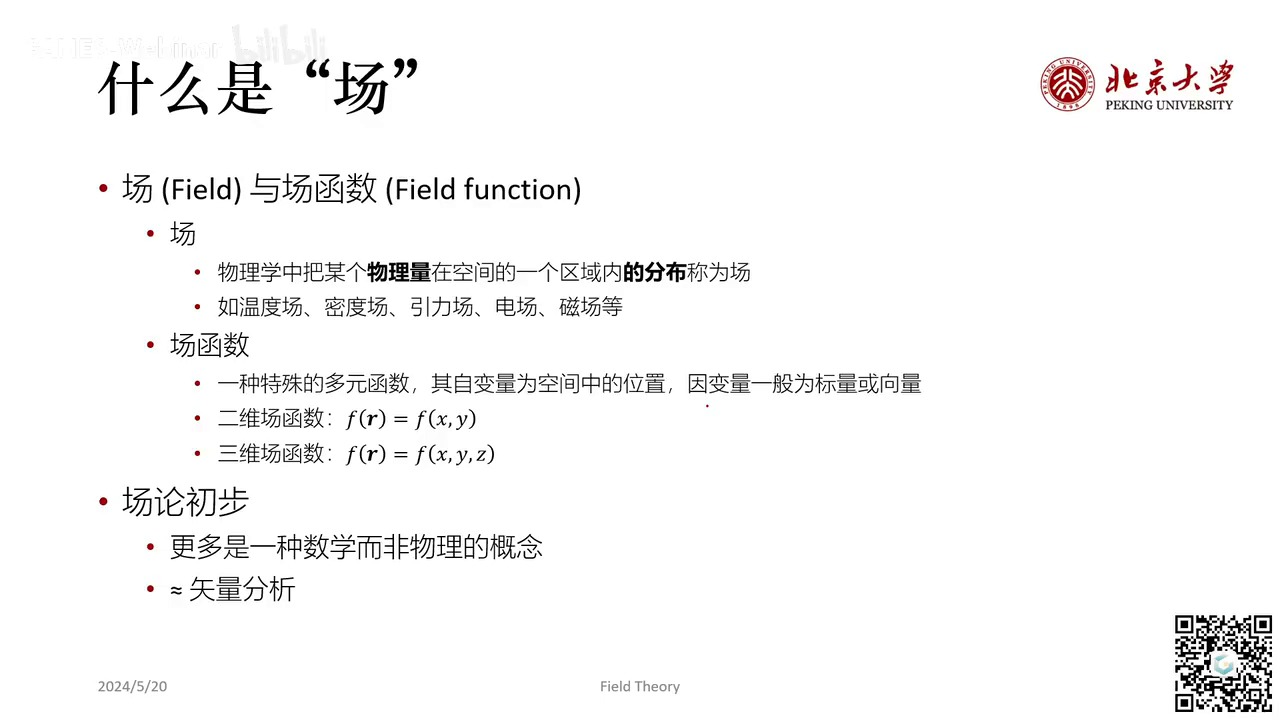
\includegraphics[width=0.92\textwidth]{figures/fig_01_field.jpg}
\caption{场与场函数的概念\vtag}
\end{figure}
\srcnote{00:00:30--00:00:45}
\end{minipage}


在物理学中，把某个物理量在空间的一个区域内的分布称为场，例如温度场、密度场、引力场、电场、磁场等。

场函数是一种特殊的多元函数：它的自变量为空间中的位置，因变量一般为标量或向量。最简单的例子是二维场函数 $f(\boldsymbol r)=f(x,y)$，其中 $\boldsymbol r$ 是二维向量，也可以展开成 $x$ 坐标和 $y$ 坐标；三维也是同理，$f(\boldsymbol r)=f(x,y,z)$。

课件特别指出：这里讲的场论初步更多是一种数学而非物理的概念，大致相当于矢量分析。

\section{标量场的梯度}

\noindent\begin{minipage}{\textwidth}
\begin{figure}[H]
\centering
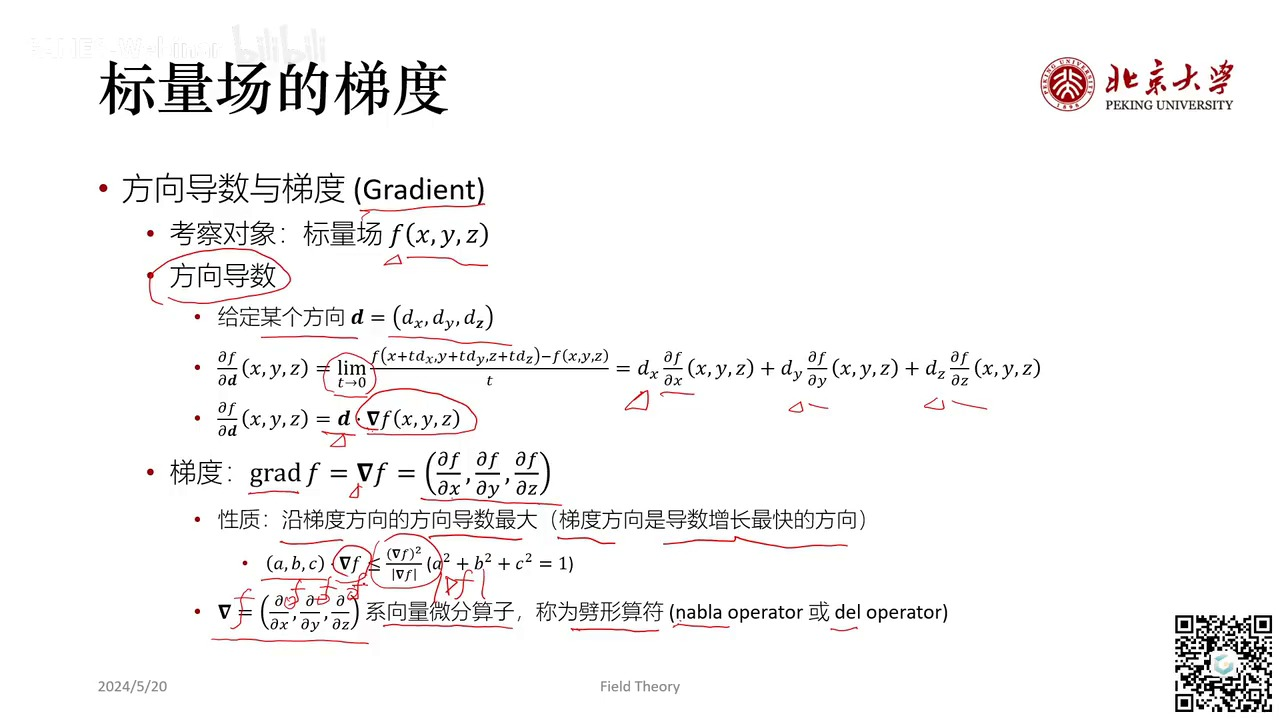
\includegraphics[width=0.92\textwidth]{figures/fig_02_gradient.jpg}
\caption{方向导数与梯度\vtag}
\end{figure}
\srcnote{00:05:45--00:06:00}
\end{minipage}


先考察最简单的场：标量场 $f(x,y,z)$。给定某个方向 $\boldsymbol d=(d_x,d_y,d_z)$，沿该方向的方向导数定义为
\begin{equation}
\frac{\partial f}{\partial\boldsymbol d}(x,y,z)=\lim_{t\to 0}\frac{f(x+td_x,y+td_y,z+td_z)-f(x,y,z)}{t}.
\end{equation}
讲者说，取极限的操作与一元函数求导数的定义是一样的。取完极限之后，根据多元函数微积分的链式法则，
\begin{equation}
\frac{\partial f}{\partial\boldsymbol d}=d_x\frac{\partial f}{\partial x}+d_y\frac{\partial f}{\partial y}+d_z\frac{\partial f}{\partial z}=\boldsymbol d\cdot\nabla f .
\end{equation}
其中
\begin{equation}
\operatorname{grad} f=\nabla f=\left(\frac{\partial f}{\partial x},\frac{\partial f}{\partial y},\frac{\partial f}{\partial z}\right)
\end{equation}
称为 $f$ 的梯度。

梯度的性质是：沿梯度方向的方向导数最大，或者说梯度方向是导数增长最快的方向。为什么？只需考察一个不等式：任取单位方向 $(a,b,c)$，即 $a^2+b^2+c^2=1$，由柯西不等式
\begin{equation}
(a,b,c)\cdot\nabla f\le\frac{(\nabla f)^2}{|\nabla f|},
\end{equation}
等号在 $(a,b,c)$ 与 $\nabla f$ 同向时取到。

\begin{knowledgebox}{哈密顿算子 $\nabla$}
讲者把梯度形式化地写成“偏 $x$ 偏什么先留个空，偏 $y$ 留个空，偏 $z$ 留个空”，即
\begin{equation}
\nabla=\left(\frac{\partial}{\partial x},\frac{\partial}{\partial y},\frac{\partial}{\partial z}\right),
\end{equation}
它是一个向量微分算子，称为劈形算符（nabla operator 或 del operator）。它作用在标量场上得到梯度；后面会看到，它与向量场做“点乘”得到散度，做“叉乘”得到旋度。
\end{knowledgebox}

\section{向量场的通量与散度}

\subsection{通量}

\noindent\begin{minipage}{\textwidth}
\begin{figure}[H]
\centering
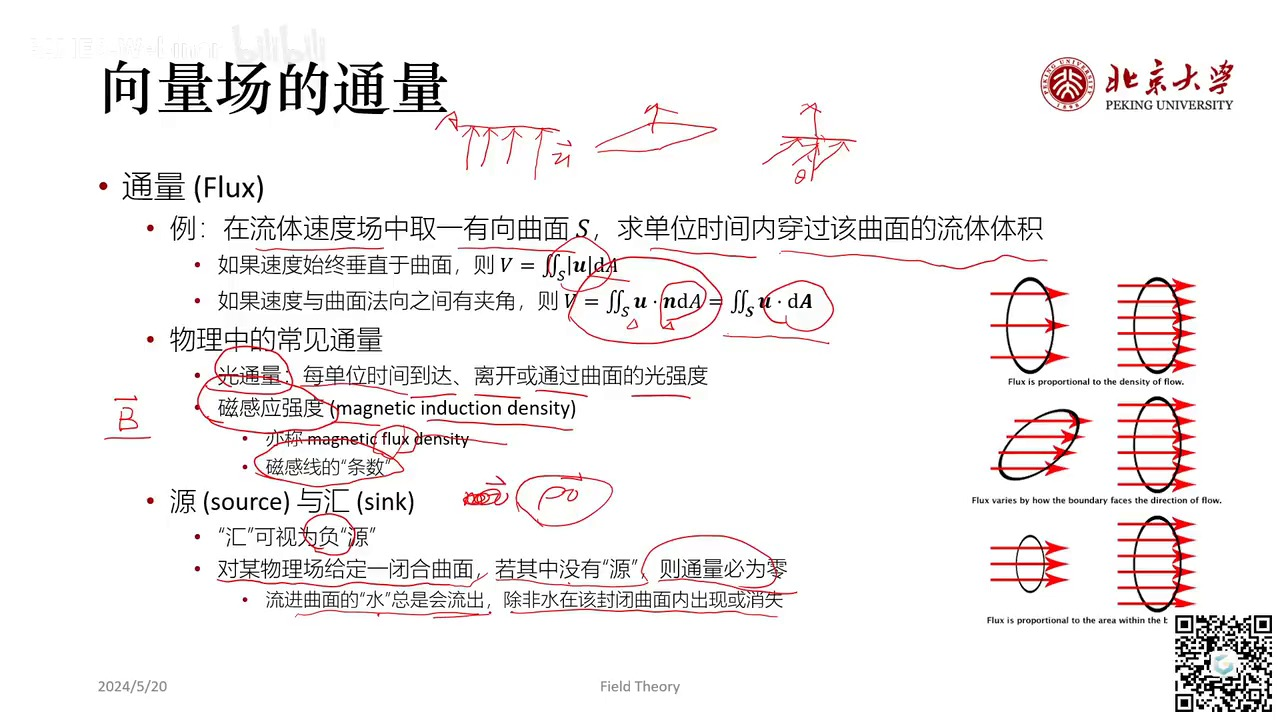
\includegraphics[width=0.92\textwidth]{figures/fig_03_flux.jpg}
\caption{向量场的通量、物理中常见的通量，以及源与汇\vtag}
\end{figure}
\srcnote{00:11:15--00:11:30}
\end{minipage}


通量的英文是 flux。例子：在流体速度场中取一个有向曲面 $S$，求单位时间内穿过该曲面的流体体积。所谓有向，是说除了曲面本身，还规定了它的正方向。如果速度始终垂直于曲面，则 $V=\iint_S|\boldsymbol u|\,\mathrm{d}A$；如果速度与曲面法向之间有夹角，则只有法向分量穿过曲面：
\begin{equation}
V=\iint_S\boldsymbol u\cdot\boldsymbol n\,\mathrm{d}A=\iint_S\boldsymbol u\cdot\mathrm{d}\boldsymbol A,
\end{equation}
其中 $\mathrm{d}\boldsymbol A$ 是方向为法向、大小为面积微元的向量。

物理中常见的通量：渲染中会接触到的光通量，即每单位时间到达、离开或通过曲面的光强度；以及磁感应强度（magnetic induction density）。讲者指出，磁感应强度还有一个英文名 magnetic flux density，即“磁通密度”，它本质上就是穿过单位面积的磁感线的“条数”。

\subsection{源与汇}

“汇”可视为负“源”。对某物理场给定一闭合曲面，若其中没有“源”，则通量必为零。讲者的比喻是：如果空间中某个地方在不停地往外生成水，用闭合曲面把它包住，就会有净的流出；而流进曲面的“水”总是会流出，除非水在该封闭曲面内出现或消失，凭空生成是不可能的。

\subsection{散度}

\noindent\begin{minipage}{\textwidth}
\begin{figure}[H]
\centering
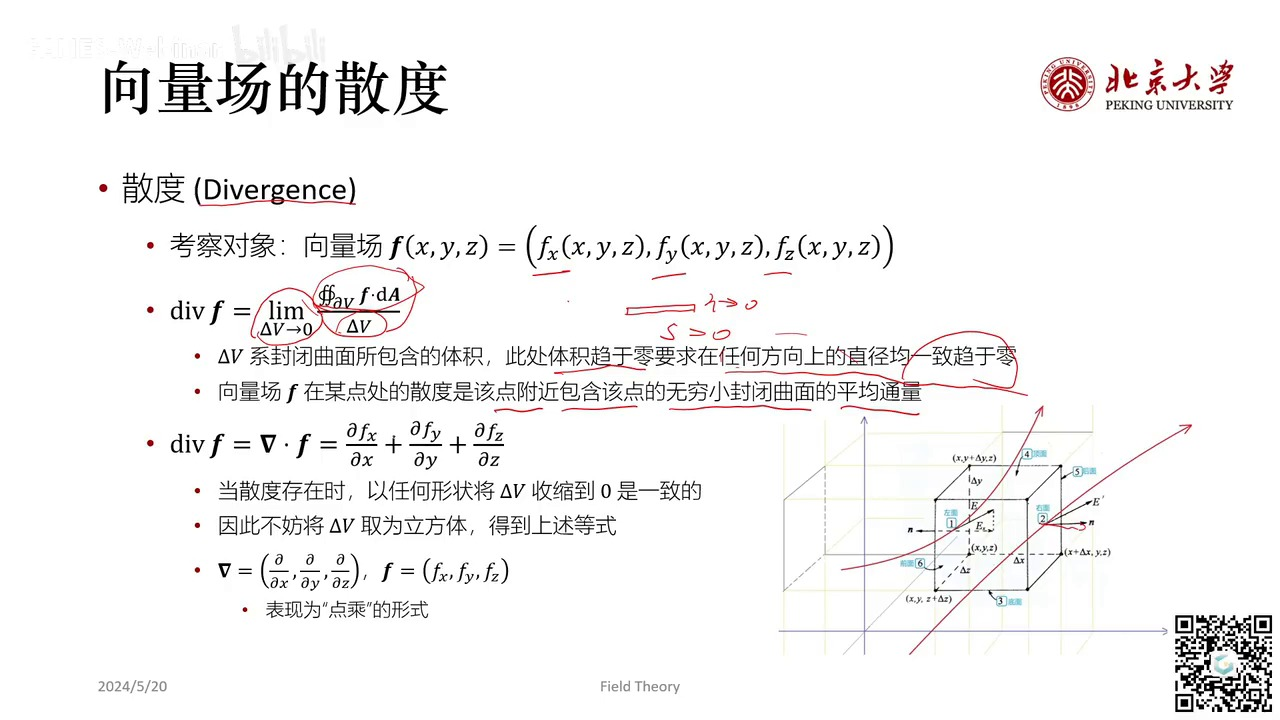
\includegraphics[width=0.92\textwidth]{figures/fig_04_divergence.jpg}
\caption{散度的定义及其在直角坐标系下的推导\vtag}
\end{figure}
\srcnote{00:13:30--00:13:45}
\end{minipage}


考察向量场 $\boldsymbol f(x,y,z)=\big(f_x(x,y,z),f_y(x,y,z),f_z(x,y,z)\big)$，定义散度为
\begin{equation}
\operatorname{div}\boldsymbol f=\lim_{\Delta V\to 0}\frac{\oint_{\partial V}\boldsymbol f\cdot\mathrm{d}\boldsymbol A}{\Delta V}.
\end{equation}
$\Delta V$ 是闭曲面所包含的体积，此处体积趋于零要求在任何方向上的直径均一致趋于零。所以向量场 $\boldsymbol f$ 在某点处的散度，是该点附近包含该点的无穷小封闭曲面的平均通量。

\begin{warningbox}{“一致趋于零”的含义}
讲者特别解释了为什么要求各方向一致趋于零：比如一个圆柱体，完全可以只把它的高无限压缩成零，而底面积仍是有限大的数。这样体积也趋于零，但闭曲面并没有收缩到一个点，不是这里所说的极限。
\end{warningbox}

在直角坐标系中如何表达？当散度存在时，以任何形状将 $\Delta V$ 收缩到零都是一致的，因此不妨将 $\Delta V$ 取为立方体，分别计算各个面上的通量，得到
\begin{equation}
\operatorname{div}\boldsymbol f=\nabla\cdot\boldsymbol f=\frac{\partial f_x}{\partial x}+\frac{\partial f_y}{\partial y}+\frac{\partial f_z}{\partial z}.
\end{equation}
它在形式上就是 $\nabla$ 与 $\boldsymbol f=(f_x,f_y,f_z)$ 的“点乘”，这也是记号中写点乘符号的原因。

\noindent\begin{minipage}{\textwidth}
\begin{figure}[H]
\centering
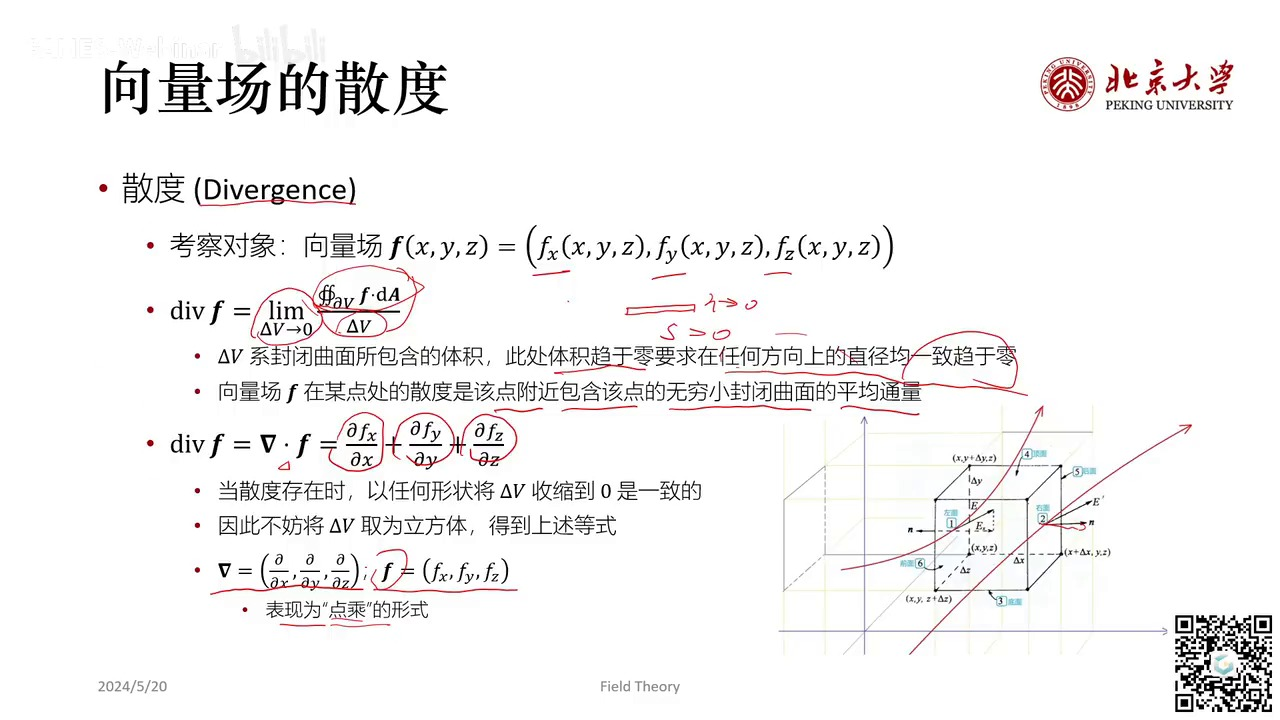
\includegraphics[width=0.92\textwidth]{figures/fig_05_divergence_note.jpg}
\caption{讲者在立方体示意图上推导散度的直角坐标表达式\vtag}
\end{figure}
\srcnote{00:14:00--00:14:15}
\end{minipage}


\subsection{散度的相对大小与高斯散度定理}

\noindent\begin{minipage}{\textwidth}
\begin{figure}[H]
\centering
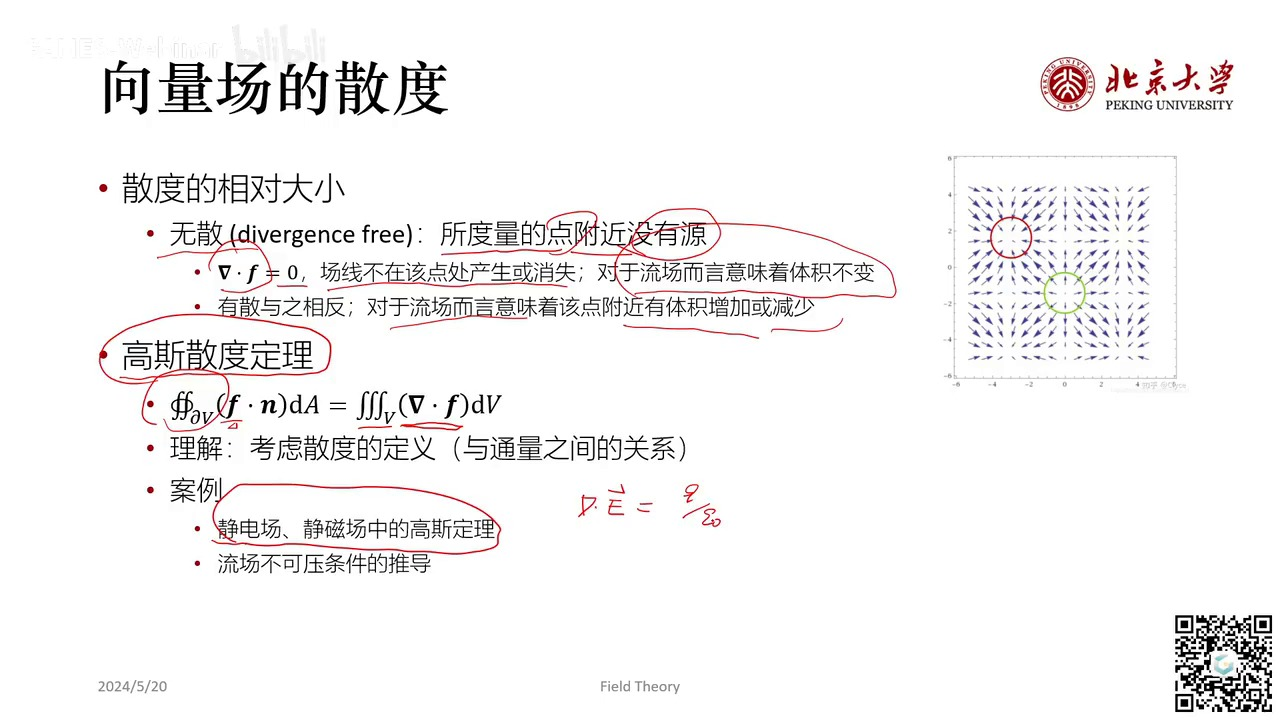
\includegraphics[width=0.92\textwidth]{figures/fig_06_gauss.jpg}
\caption{无散场、高斯散度定理及其物理案例\vtag}
\end{figure}
\srcnote{00:17:45--00:18:00}
\end{minipage}


无散（divergence free）是说所度量的点附近没有源，记作 $\nabla\cdot\boldsymbol f=0$。它的意思是场线不在该点处产生或消失；对于流场而言，意味着体积不变。有散则相反，对于流场而言，意味着该点附近有体积增加或减少。

讲者结合右图解释：绿色圈所包含的地方，水都是从里面往外流的，说明这里有源。如果把圈不断缩小，缩小到半径为零，就得到这一点的散度。把一块体积分成无数小块，相邻小块共享的面上通量一进一出相互抵消，只剩下最外面的表面，于是不太严格地推出了高斯散度定理：
\begin{equation}
\oint_{\partial V}(\boldsymbol f\cdot\boldsymbol n)\,\mathrm{d}A=\iiint_V(\nabla\cdot\boldsymbol f)\,\mathrm{d}V .
\end{equation}
它的意思是：给定空间中任意一块体积，体积内向量场散度的积分，等于在体积表面上求向量场的通量。理解它的关键是散度的定义与通量之间的关系。

\begin{practicebox}{高斯定理的三个案例}
课件列出的案例，读者可以对照上式理解：
\begin{enumerate}
\item 静电场的高斯定理：闭合曲面上电场强度的通量，等于曲面内包含的电荷量乘以因子 $1/\varepsilon_0$。
\item 静磁场的高斯定理：磁场没有可以产生或消失的地方，所以任意闭合曲面上的磁通量为零。
\item 流场不可压条件：流体不可压时，任一块体积不增多也不减少，所以速度场的散度为零，$\nabla\cdot\boldsymbol u=0$。这是流体模拟中最重要的约束之一。
\end{enumerate}
\end{practicebox}

\section{向量场的环量与旋度}

\subsection{环量}

\noindent\begin{minipage}{\textwidth}
\begin{figure}[H]
\centering
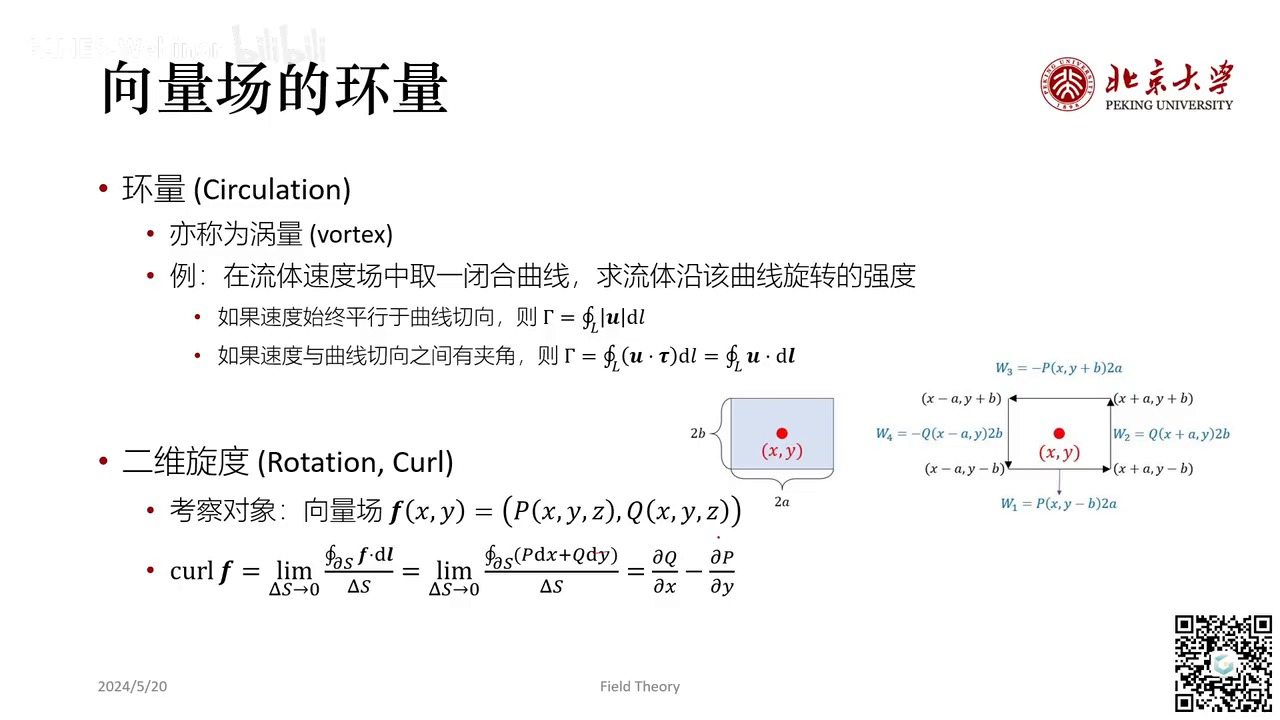
\includegraphics[width=0.92\textwidth]{figures/fig_07_circulation.jpg}
\caption{环量与二维旋度\vtag}
\end{figure}
\srcnote{00:20:00--00:20:15}
\end{minipage}


环量（circulation）也称为涡量（vortex）。最直观的例子是：在流体速度场中取一条闭合曲线，求流体沿该曲线旋转的强度。如果速度始终平行于曲线切向，则 $\Gamma=\oint_L|\boldsymbol u|\,\mathrm{d}l$；如果速度与曲线切向之间有夹角，就取切向分量：
\begin{equation}
\Gamma=\oint_L(\boldsymbol u\cdot\boldsymbol\tau)\,\mathrm{d}l=\oint_L\boldsymbol u\cdot\mathrm{d}\boldsymbol l .
\end{equation}

\subsection{二维旋度}

旋度记作 rotation 或 curl。先看二维：考察向量场 $\boldsymbol f(x,y)=\big(P(x,y),Q(x,y)\big)$。在二维平面上任画一条闭合曲线，它围成面积 $\Delta S$；与散度一样，当面积在各个方向上一致趋于零时，
\begin{equation}
\operatorname{curl}\boldsymbol f=\lim_{\Delta S\to 0}\frac{\oint_{\partial S}\boldsymbol f\cdot\mathrm{d}\boldsymbol l}{\Delta S}=\lim_{\Delta S\to 0}\frac{\oint_{\partial S}(P\,\mathrm{d}x+Q\,\mathrm{d}y)}{\Delta S}=\frac{\partial Q}{\partial x}-\frac{\partial P}{\partial y}.
\end{equation}

\noindent\begin{minipage}{\textwidth}
\begin{figure}[H]
\centering
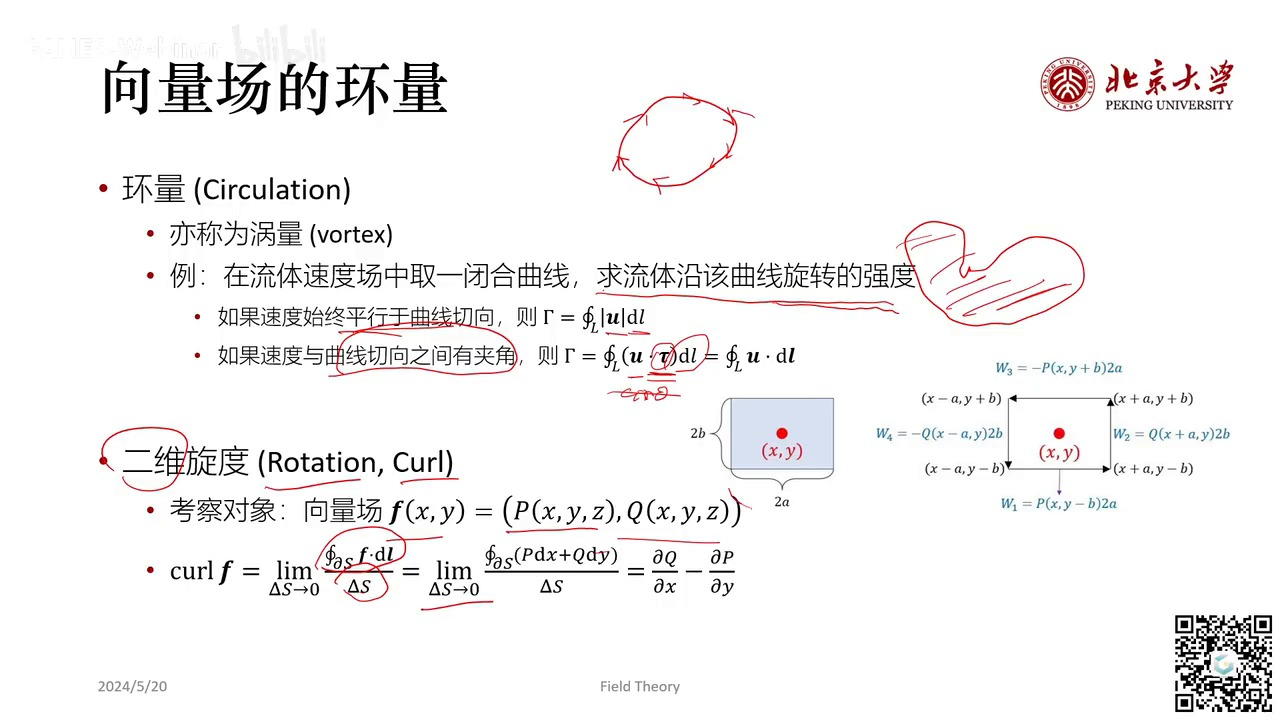
\includegraphics[width=0.92\textwidth]{figures/fig_08_circulation_note.jpg}
\caption{讲者在小矩形回路上逐边计算环量\vtag}
\end{figure}
\srcnote{00:22:45--00:23:00}
\end{minipage}


计算时取以 $(x,y)$ 为中心、边长为 $2a$ 和 $2b$ 的小矩形，一条边一条边地算环量：上边贡献 $-P(x,y+b)\,2a$，下边贡献 $P(x,y-b)\,2a$，右边贡献 $Q(x+a,y)\,2b$，左边贡献 $-Q(x-a,y)\,2b$。加起来再除以面积 $4ab$，取极限，就得到 $\partial Q/\partial x-\partial P/\partial y$。

\subsection{三维旋度}

\noindent\begin{minipage}{\textwidth}
\begin{figure}[H]
\centering
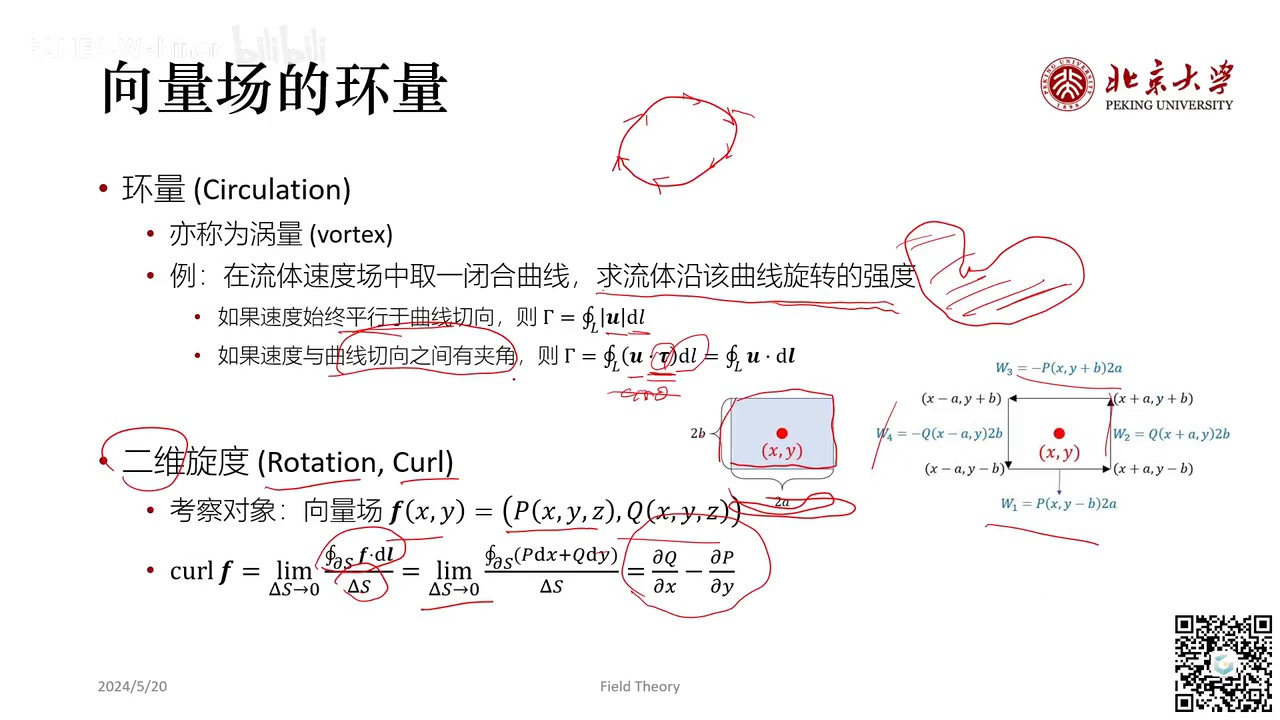
\includegraphics[width=0.92\textwidth]{figures/fig_09_curl3d.jpg}
\caption{三维旋度：沿三个坐标方向的面元分别计算\vtag}
\end{figure}
\srcnote{00:23:45--00:24:00}
\end{minipage}


对三维向量场 $\boldsymbol f(x,y,z)=\big(P,Q,R\big)$，分别在法向沿 $x,y,z$ 方向的面元 $S_x,S_y,S_z$ 上计算：
\begin{equation}
\operatorname{curl}\boldsymbol f=\operatorname{rot}\boldsymbol f=\left(\lim_{\Delta S_x\to 0}\frac{\oint_{\partial S_x}\boldsymbol f\cdot\mathrm{d}\boldsymbol l}{\Delta S_x},\ \lim_{\Delta S_y\to 0}\frac{\oint_{\partial S_y}\boldsymbol f\cdot\mathrm{d}\boldsymbol l}{\Delta S_y},\ \lim_{\Delta S_z\to 0}\frac{\oint_{\partial S_z}\boldsymbol f\cdot\mathrm{d}\boldsymbol l}{\Delta S_z}\right).
\end{equation}
讲者解释：$xOy$ 平面的法向指向 $z$ 方向，所以刚才二维情形算出的正是 $z$ 分量；再把其余各个回路都算一下，得到
\begin{equation}
\operatorname{curl}\boldsymbol f=\left(\frac{\partial R}{\partial y}-\frac{\partial Q}{\partial z},\ \frac{\partial P}{\partial z}-\frac{\partial R}{\partial x},\ \frac{\partial Q}{\partial x}-\frac{\partial P}{\partial y}\right)=\nabla\times\boldsymbol f .
\end{equation}
它在形式上就等于 $\nabla$ 叉乘 $\boldsymbol f$。

\subsection{格林公式与斯托克斯定理}

\noindent\begin{minipage}{\textwidth}
\begin{figure}[H]
\centering
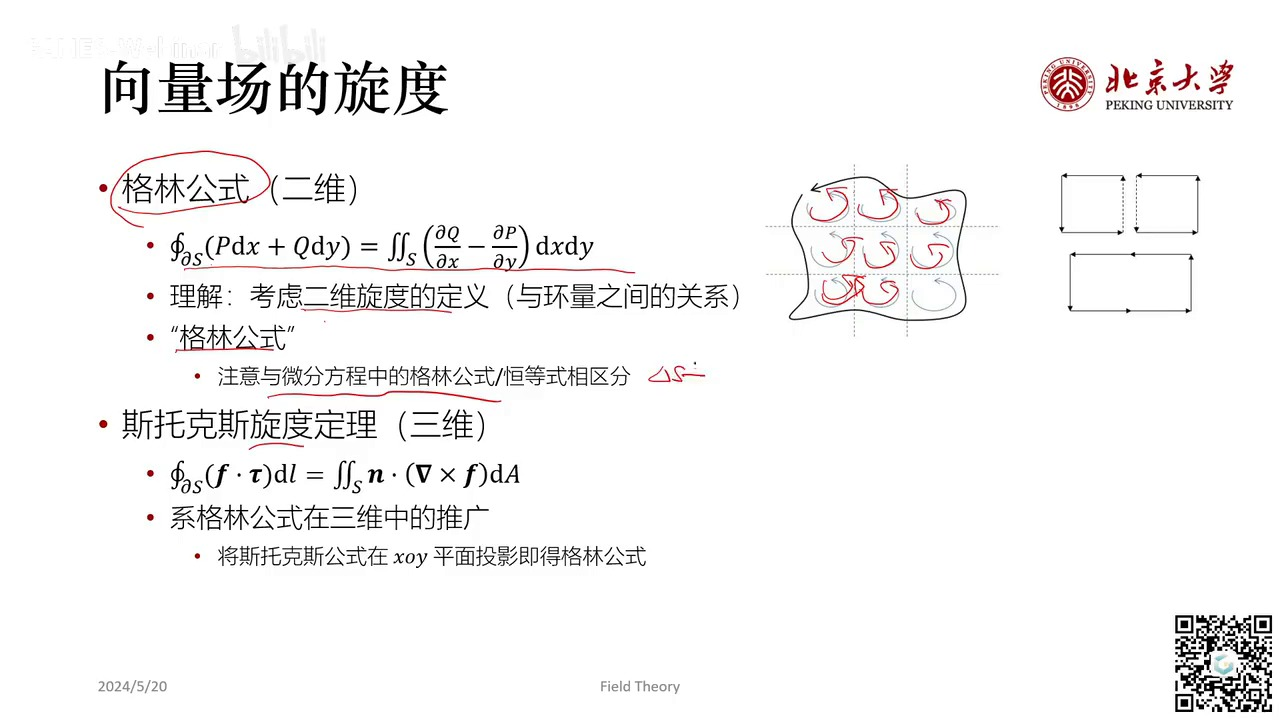
\includegraphics[width=0.92\textwidth]{figures/fig_10_green.jpg}
\caption{格林公式与斯托克斯旋度定理\vtag}
\end{figure}
\srcnote{00:26:30--00:26:45}
\end{minipage}


推导二维旋度时得到的结果，本身又称为格林公式：
\begin{equation}
\oint_{\partial S}(P\,\mathrm{d}x+Q\,\mathrm{d}y)=\iint_S\left(\frac{\partial Q}{\partial x}-\frac{\partial P}{\partial y}\right)\mathrm{d}x\,\mathrm{d}y .
\end{equation}
理解它的关键是二维旋度的定义与环量之间的关系。讲者在图上解释：把区域分成无限个小方格，每个小方格的旋度都是一个环量。相邻两个小方格共享的边上，左边方格的环量在这条边上朝上，右边方格的环量朝下，正好抵消。所有内部的边都抵消掉，就只剩下最外面的一环。

\begin{warningbox}{两个“格林公式”}
讲者提醒，这里的格林公式与微分方程中的格林公式（格林恒等式）不是一回事，后者会在之后讲偏微分方程时遇到。
\end{warningbox}

三维中的推广是斯托克斯旋度定理：
\begin{equation}
\oint_{\partial S}(\boldsymbol f\cdot\boldsymbol\tau)\,\mathrm{d}l=\iint_S\boldsymbol n\cdot(\nabla\times\boldsymbol f)\,\mathrm{d}A .
\end{equation}
在三维中曲面可以朝向任意方向，所以需要加上与法向量的点乘。若将斯托克斯公式在 $xOy$ 平面上投影，立刻就得到格林公式。

\section{矢量微分恒等式与位矢}

\subsection{拉普拉斯算子}

\noindent\begin{minipage}{\textwidth}
\begin{figure}[H]
\centering
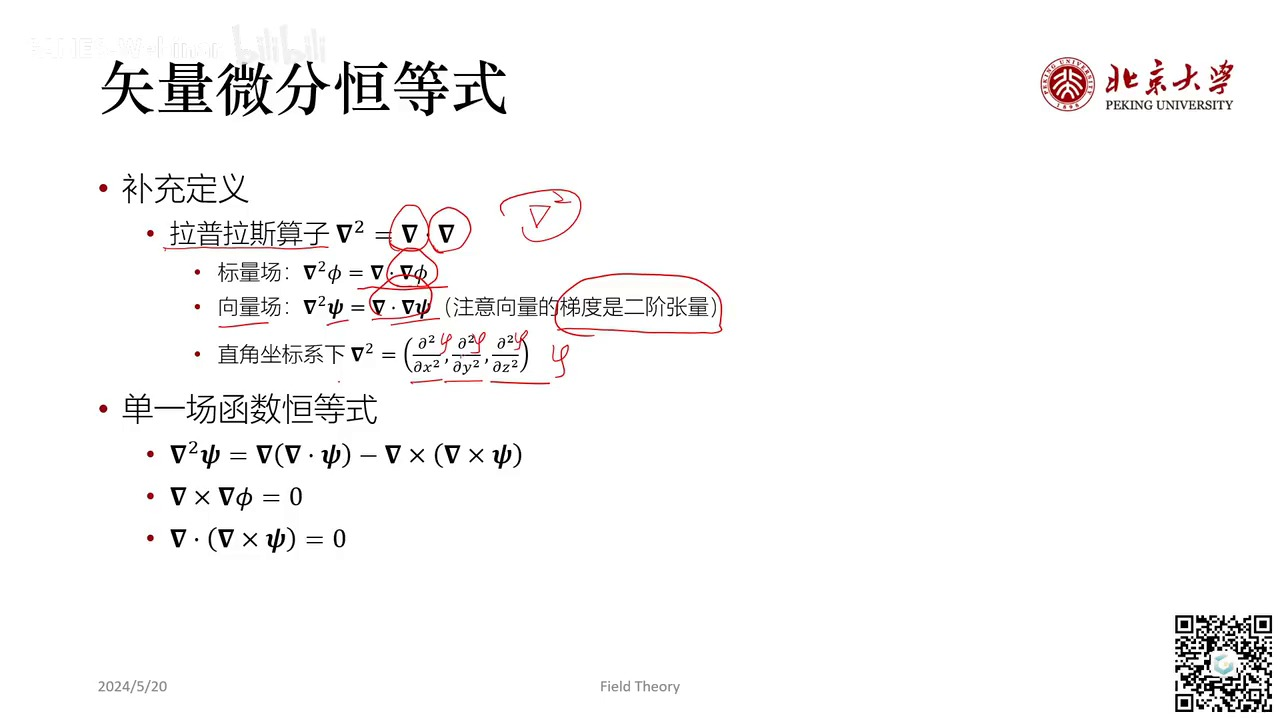
\includegraphics[width=0.92\textwidth]{figures/fig_11_identities.jpg}
\caption{拉普拉斯算子与单一场函数恒等式\vtag}
\end{figure}
\srcnote{00:29:45--00:30:00}
\end{minipage}


补充定义拉普拉斯算子 $\nabla^2=\nabla\cdot\nabla$。对标量场，$\nabla^2\phi=\nabla\cdot\nabla\phi$：先求梯度变成矢量场，再求散度又变回标量。对向量场，$\nabla^2\boldsymbol\psi=\nabla\cdot\nabla\boldsymbol\psi$，注意向量的梯度是二阶张量，二阶张量再求散度，结果还是矢量。在直角坐标系下，
\begin{equation}
\nabla^2=\frac{\partial^2}{\partial x^2}+\frac{\partial^2}{\partial y^2}+\frac{\partial^2}{\partial z^2}.
\end{equation}

\begin{warningbox}{课件上的写法}
课件把直角坐标下的 $\nabla^2$ 写成了一个三元组 $\left(\frac{\partial^2}{\partial x^2},\frac{\partial^2}{\partial y^2},\frac{\partial^2}{\partial z^2}\right)$。讲者在课上说要改一下：$\nabla^2$ 是 $\nabla$ 与自身的点乘，是一个标量算子，应写成上式的求和形式。
\end{warningbox}

\subsection{单一场函数恒等式}

\begin{equation}
\begin{gathered}
\nabla^2\boldsymbol\psi=\nabla(\nabla\cdot\boldsymbol\psi)-\nabla\times(\nabla\times\boldsymbol\psi),\\
\nabla\times\nabla\phi=\boldsymbol 0,\qquad \nabla\cdot(\nabla\times\boldsymbol\psi)=0 .
\end{gathered}
\end{equation}
后两条是说：标量场梯度的旋度一定为零，矢量场旋度的散度也一定为零。讲者强调这两个式子非常重要，一会儿证明亥姆霍兹分解时需要用到；它们的证明留到最后用外微分来做。

\subsection{多场函数恒等式}

\noindent\begin{minipage}{\textwidth}
\begin{figure}[H]
\centering
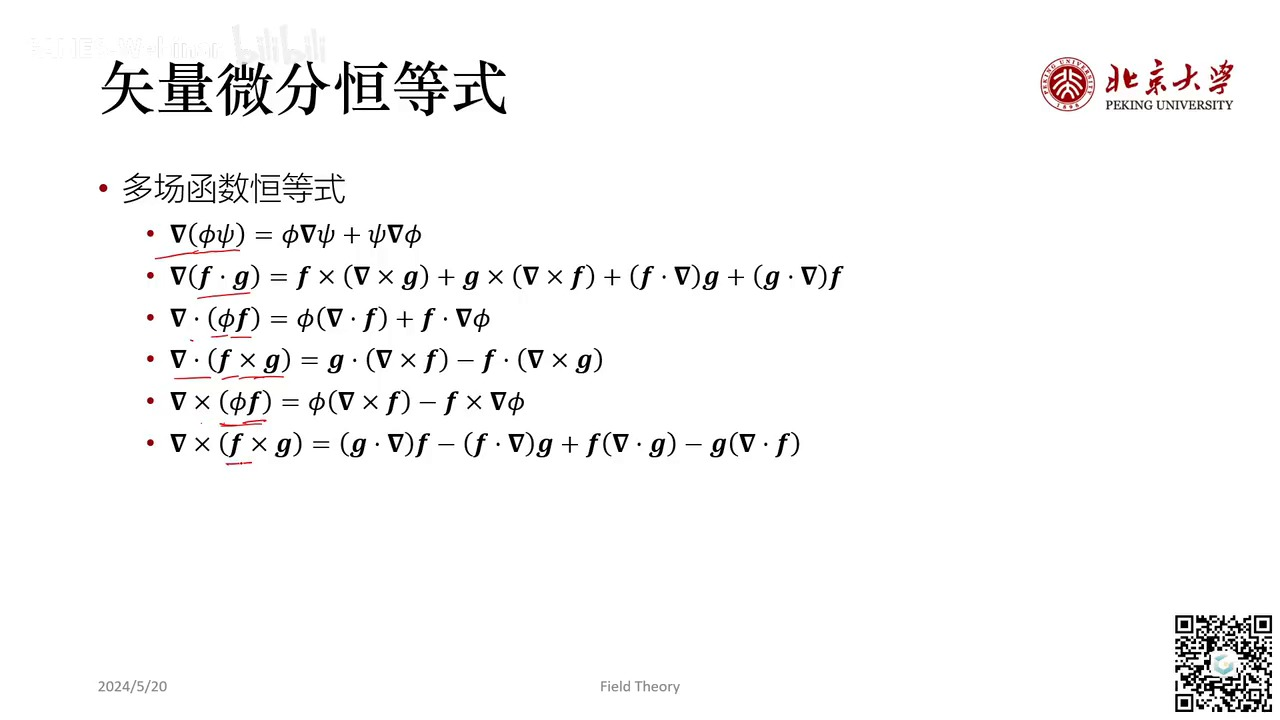
\includegraphics[width=0.92\textwidth]{figures/fig_12_identities_multi.jpg}
\caption{多场函数的矢量微分恒等式\vtag}
\end{figure}
\srcnote{00:32:30--00:32:45}
\end{minipage}


讲者说，他把常见的矢量微分恒等式基本都列在课件上了，以后需要时当表查就可以：
\begin{equation}
\begin{gathered}
\nabla(\phi\psi)=\phi\nabla\psi+\psi\nabla\phi,\\
\nabla(\boldsymbol f\cdot\boldsymbol g)=\boldsymbol f\times(\nabla\times\boldsymbol g)+\boldsymbol g\times(\nabla\times\boldsymbol f)+(\boldsymbol f\cdot\nabla)\boldsymbol g+(\boldsymbol g\cdot\nabla)\boldsymbol f,\\
\nabla\cdot(\phi\boldsymbol f)=\phi(\nabla\cdot\boldsymbol f)+\boldsymbol f\cdot\nabla\phi,\\
\nabla\cdot(\boldsymbol f\times\boldsymbol g)=\boldsymbol g\cdot(\nabla\times\boldsymbol f)-\boldsymbol f\cdot(\nabla\times\boldsymbol g),\\
\nabla\times(\phi\boldsymbol f)=\phi(\nabla\times\boldsymbol f)-\boldsymbol f\times\nabla\phi,\\
\nabla\times(\boldsymbol f\times\boldsymbol g)=(\boldsymbol g\cdot\nabla)\boldsymbol f-(\boldsymbol f\cdot\nabla)\boldsymbol g+\boldsymbol f(\nabla\cdot\boldsymbol g)-\boldsymbol g(\nabla\cdot\boldsymbol f).
\end{gathered}
\end{equation}

\subsection{位矢：特殊的场函数}

\noindent\begin{minipage}{\textwidth}
\begin{figure}[H]
\centering
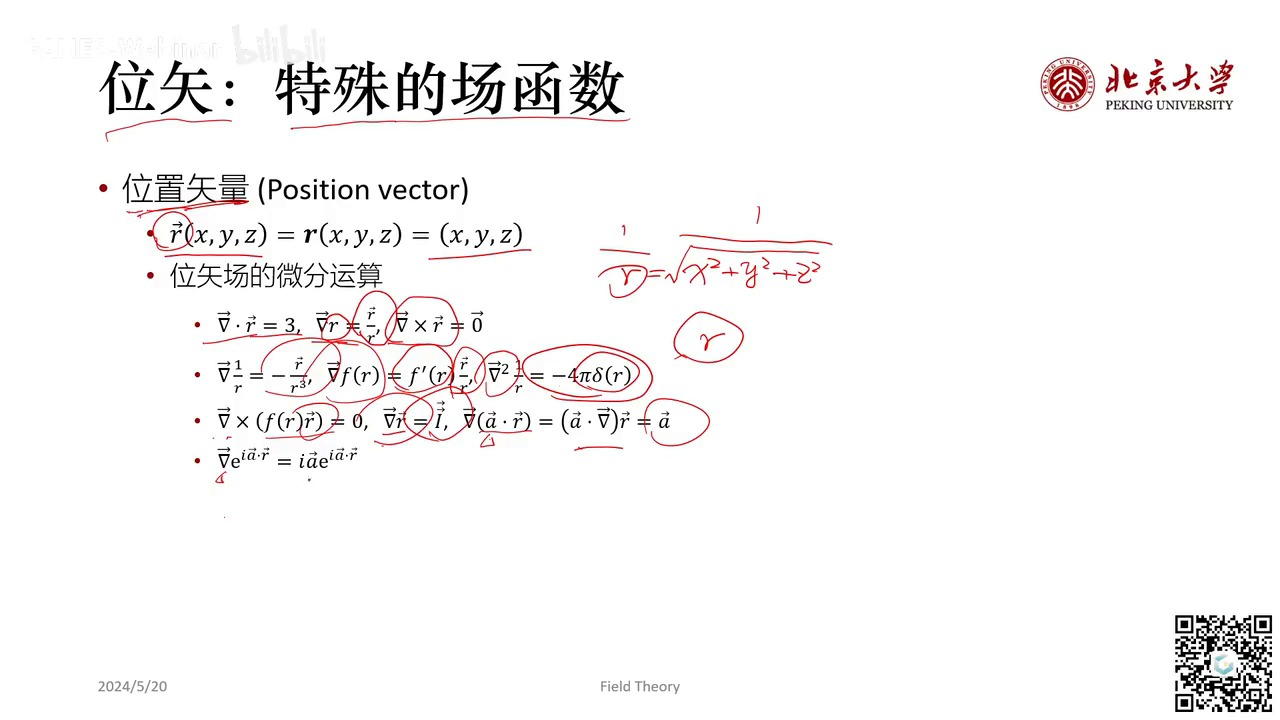
\includegraphics[width=0.92\textwidth]{figures/fig_13_position.jpg}
\caption{位置矢量及其微分运算\vtag}
\end{figure}
\srcnote{00:35:45--00:36:00}
\end{minipage}


位置矢量 $\vec r(x,y,z)=\boldsymbol r(x,y,z)=(x,y,z)$。讲者说明，这里用带箭头的手写体表示矢量，是因为接下来既要出现矢量 $\vec r$，又要出现标量 $r=|\vec r|$，以免混淆。位矢场的常用微分运算有
\begin{equation}
\begin{gathered}
\nabla\cdot\vec r=3,\qquad \nabla r=\frac{\vec r}{r},\qquad \nabla\times\vec r=\vec 0,\\
\nabla\frac{1}{r}=-\frac{\vec r}{r^3},\qquad \nabla f(r)=f'(r)\frac{\vec r}{r},\qquad \nabla^2\frac{1}{r}=-4\pi\delta(\vec r),\\
\nabla\times\big(f(r)\vec r\big)=\vec 0,\qquad \nabla\vec r=\overleftrightarrow{I},\qquad \nabla(\vec a\cdot\vec r)=(\vec a\cdot\nabla)\vec r=\vec a,\qquad \nabla e^{i\vec a\cdot\vec r}=i\vec a\,e^{i\vec a\cdot\vec r}.
\end{gathered}
\end{equation}
讲者逐条解释：$\nabla r$ 得到的是 $\vec r$ 所对应的方向向量；位矢的旋度为零；把位矢的大小 $r$ 作为自变量放进函数里，梯度沿径向；位矢直接求梯度得到的是张量，即单位张量；任取常矢量 $\vec a$ 与位矢点乘再求梯度，得到 $\vec a$ 本身。

\begin{knowledgebox}{$\nabla^2(1/r)$ 中的 Delta 函数}
讲义作者补充：在 $r\ne 0$ 处可以直接验证 $\nabla^2(1/r)=0$；但在原点 $1/r$ 是奇异的。用高斯定理在包住原点的小球面上计算 $\nabla(1/r)$ 的通量，结果恒为 $-4\pi$，与球的大小无关，所以它的“散度”集中在原点，写成 $-4\pi\delta(\vec r)$。这正是点电荷电场的数学描述。
\end{knowledgebox}

\section{亥姆霍兹分解}

讲完矢量微积分的基本知识，讲者开始介绍矢量分析中非常重要的定理：亥姆霍兹分解（Helmholtz decomposition）。

\subsection{引理一：无源场}

\noindent\begin{minipage}{\textwidth}
\begin{figure}[H]
\centering
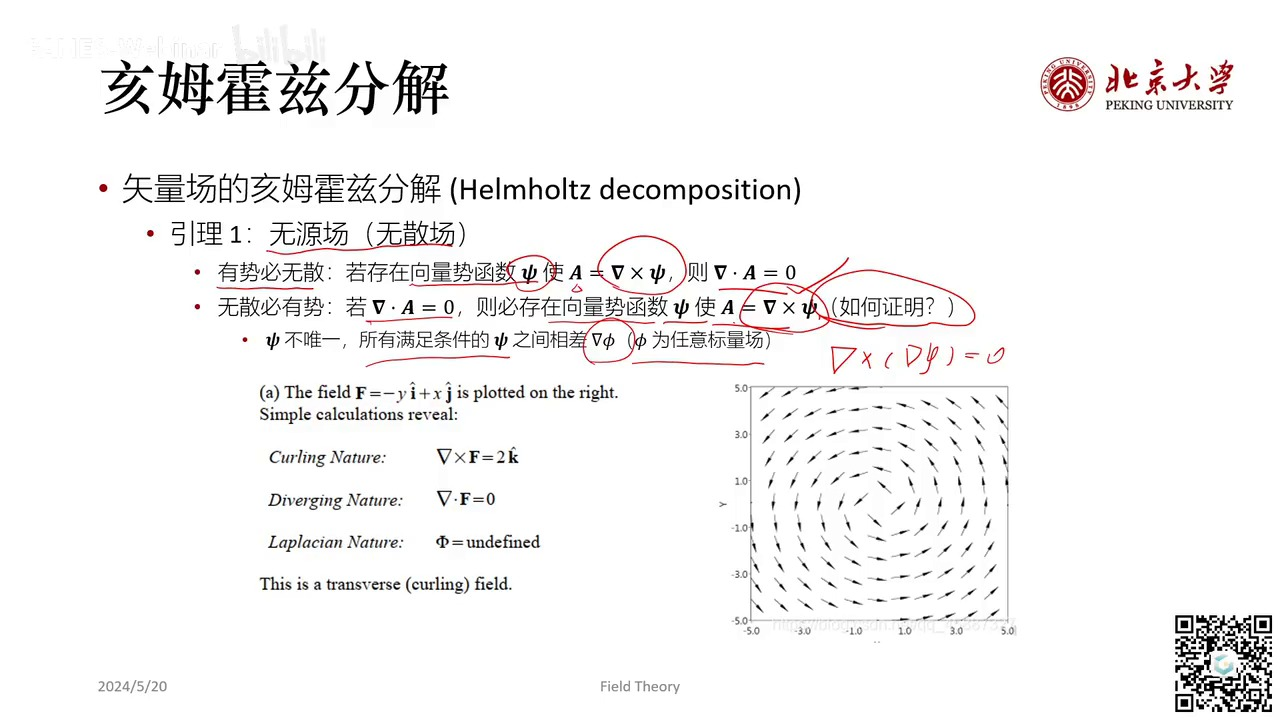
\includegraphics[width=0.92\textwidth]{figures/fig_14_helmholtz1.jpg}
\caption{引理一：无源场与例 (a) 纯旋转场\vtag}
\end{figure}
\srcnote{00:38:00--00:38:15}
\end{minipage}


无源场也称无散场。引理一有两层意思。有势必无散：若存在向量势函数 $\boldsymbol\psi$ 使 $\boldsymbol A=\nabla\times\boldsymbol\psi$，则 $\nabla\cdot\boldsymbol A=0$，这正是刚才的恒等式。无散必有势：若 $\nabla\cdot\boldsymbol A=0$，则必存在向量势函数 $\boldsymbol\psi$ 使 $\boldsymbol A=\nabla\times\boldsymbol\psi$。讲者说后一条的证明涉及微分方程的知识，感兴趣的同学可以课后了解。

需要说明的是 $\boldsymbol\psi$ 不唯一：所有满足条件的 $\boldsymbol\psi$ 之间相差 $\nabla\phi$，其中 $\phi$ 为任意标量场，因为梯度的旋度为零。课件的例 (a) 是 $\boldsymbol F=-y\boldsymbol i+x\boldsymbol j$，计算可得 $\nabla\times\boldsymbol F=2\boldsymbol k$，$\nabla\cdot\boldsymbol F=0$，这是一个纯旋转（横向）场。

\subsection{引理二：无旋场}

\noindent\begin{minipage}{\textwidth}
\begin{figure}[H]
\centering
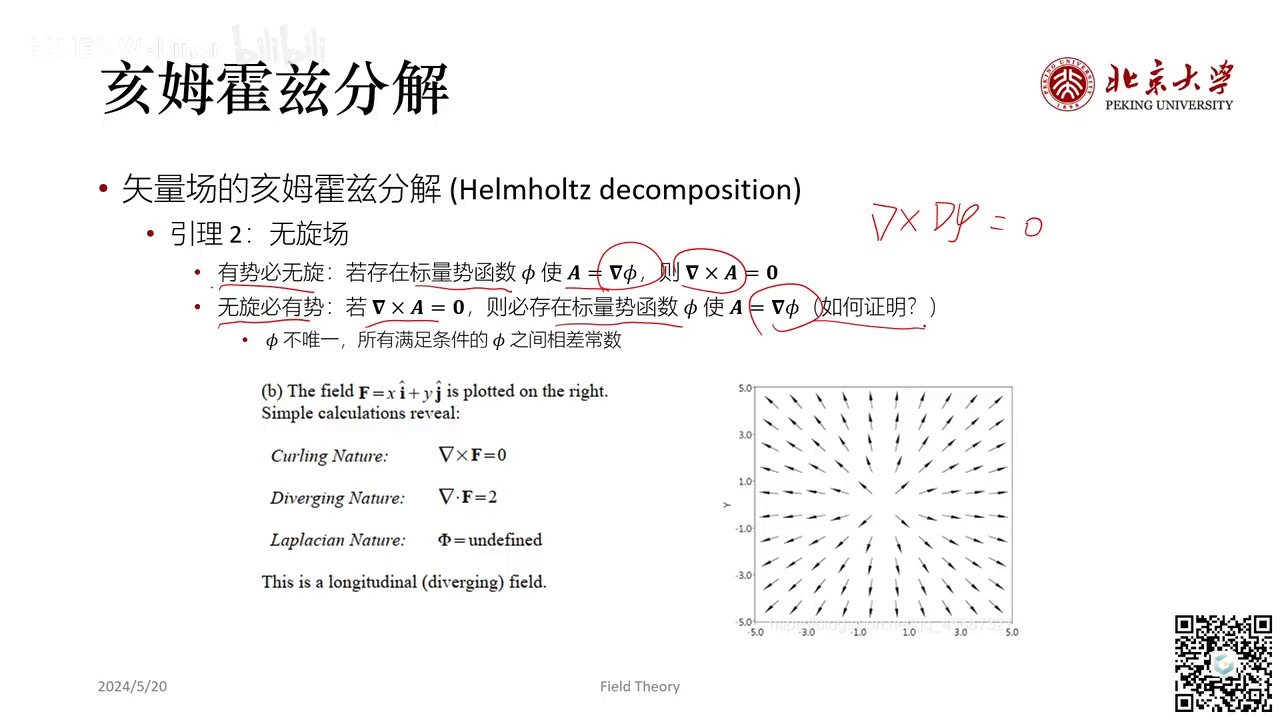
\includegraphics[width=0.92\textwidth]{figures/fig_15_helmholtz2.jpg}
\caption{引理二：无旋场与例 (b) 纯发散场\vtag}
\end{figure}
\srcnote{00:38:45--00:39:00}
\end{minipage}


引理二是对无旋场而言的。有势必无旋：若存在标量势函数 $\phi$ 使 $\boldsymbol A=\nabla\phi$，则 $\nabla\times\boldsymbol A=\boldsymbol 0$。无旋必有势：若 $\nabla\times\boldsymbol A=\boldsymbol 0$，则必存在标量势函数 $\phi$ 使 $\boldsymbol A=\nabla\phi$。这里 $\phi$ 也不唯一，所有满足条件的 $\phi$ 之间相差常数，因为常数在求梯度时不参与计算。课件的例 (b) 是 $\boldsymbol F=x\boldsymbol i+y\boldsymbol j$：$\nabla\times\boldsymbol F=\boldsymbol 0$，$\nabla\cdot\boldsymbol F=2$，这是纯发散（纵向）场。

\subsection{推论：无旋无源场}

\noindent\begin{minipage}{\textwidth}
\begin{figure}[H]
\centering
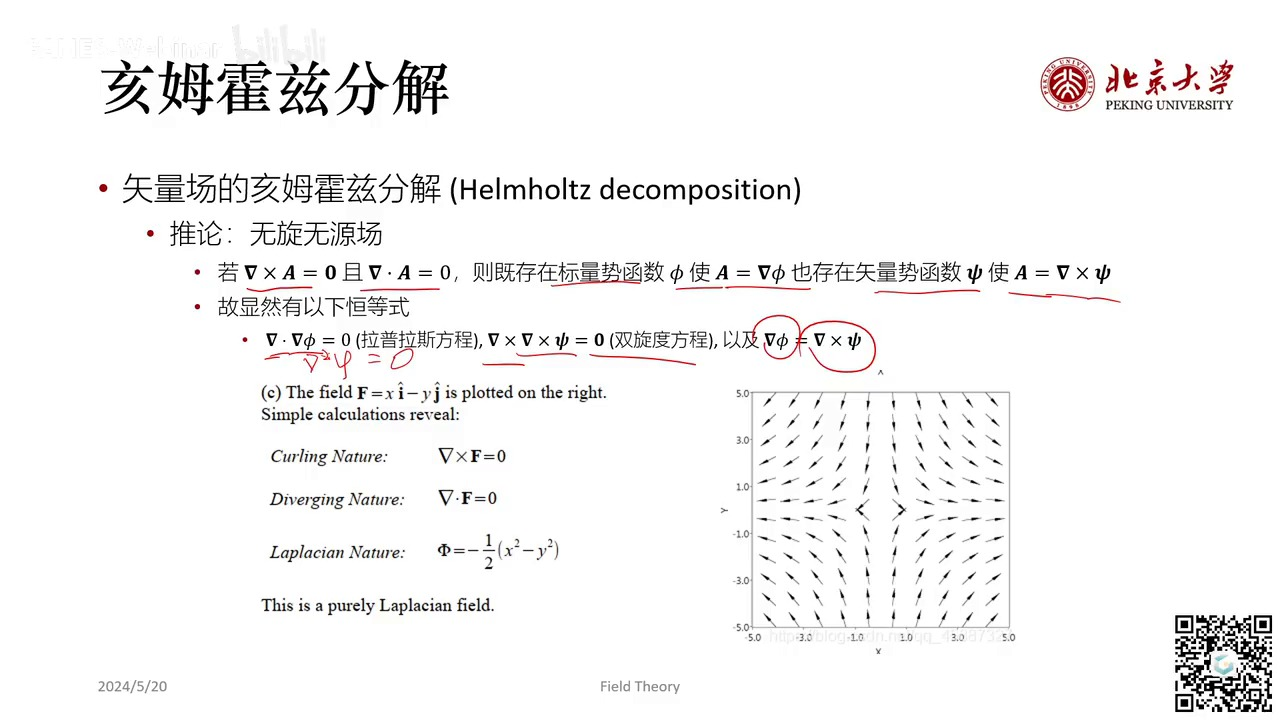
\includegraphics[width=0.92\textwidth]{figures/fig_16_helmholtz3.jpg}
\caption{推论：无旋无源场与例 (c) 拉普拉斯场\vtag}
\end{figure}
\srcnote{00:40:00--00:40:15}
\end{minipage}


若 $\nabla\times\boldsymbol A=\boldsymbol 0$ 且 $\nabla\cdot\boldsymbol A=0$，则既存在标量势函数 $\phi$ 使 $\boldsymbol A=\nabla\phi$，也存在向量势函数 $\boldsymbol\psi$ 使 $\boldsymbol A=\nabla\times\boldsymbol\psi$。此时显然有
\begin{equation}
\nabla\cdot\nabla\phi=\nabla^2\phi=0,\qquad \nabla\times\nabla\times\boldsymbol\psi=\boldsymbol 0 .
\end{equation}
前者是拉普拉斯方程，后者是双旋度方程，以及 $\nabla\phi=\nabla\times\boldsymbol\psi$。例 (c) 是 $\boldsymbol F=x\boldsymbol i-y\boldsymbol j$：旋度、散度都为零，势函数 $\Phi=-\frac{1}{2}(x^2-y^2)$，是一个纯拉普拉斯场。

\subsection{结论：有旋有源场}

\noindent\begin{minipage}{\textwidth}
\begin{figure}[H]
\centering
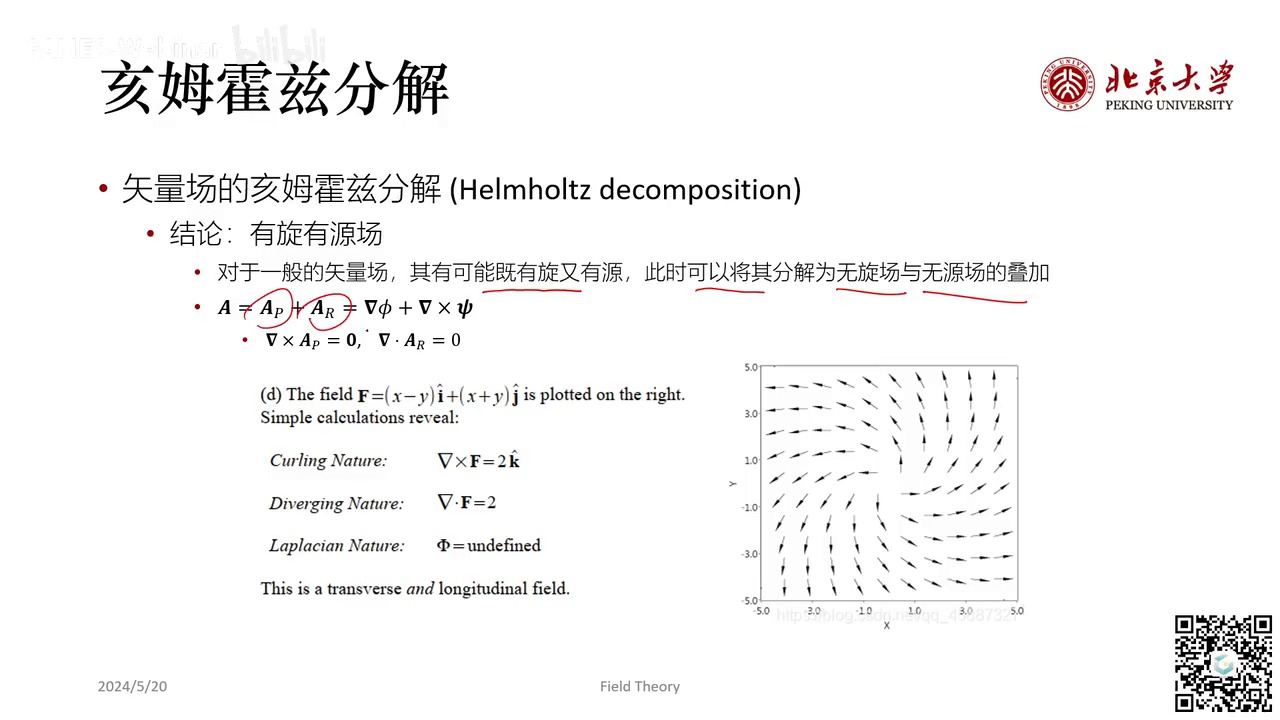
\includegraphics[width=0.92\textwidth]{figures/fig_17_helmholtz4.jpg}
\caption{结论：一般向量场分解为无旋场与无源场之和，例 (d)\vtag}
\end{figure}
\srcnote{00:40:30--00:40:45}
\end{minipage}


对于一般的矢量场，有可能既有旋又有源。此时可以将其分解为无旋场与无源场的叠加：
\begin{equation}
\boldsymbol A=\boldsymbol A_P+\boldsymbol A_R=\nabla\phi+\nabla\times\boldsymbol\psi,\qquad \nabla\times\boldsymbol A_P=\boldsymbol 0,\quad \nabla\cdot\boldsymbol A_R=0 .
\end{equation}
例 (d) 是 $\boldsymbol F=(x-y)\boldsymbol i+(x+y)\boldsymbol j$：$\nabla\times\boldsymbol F=2\boldsymbol k$，$\nabla\cdot\boldsymbol F=2$，既是横向场也是纵向场，可以看成例 (a) 与例 (b) 之和。

\subsection{存在性、唯一性与规范化}

\noindent\begin{minipage}{\textwidth}
\begin{figure}[H]
\centering
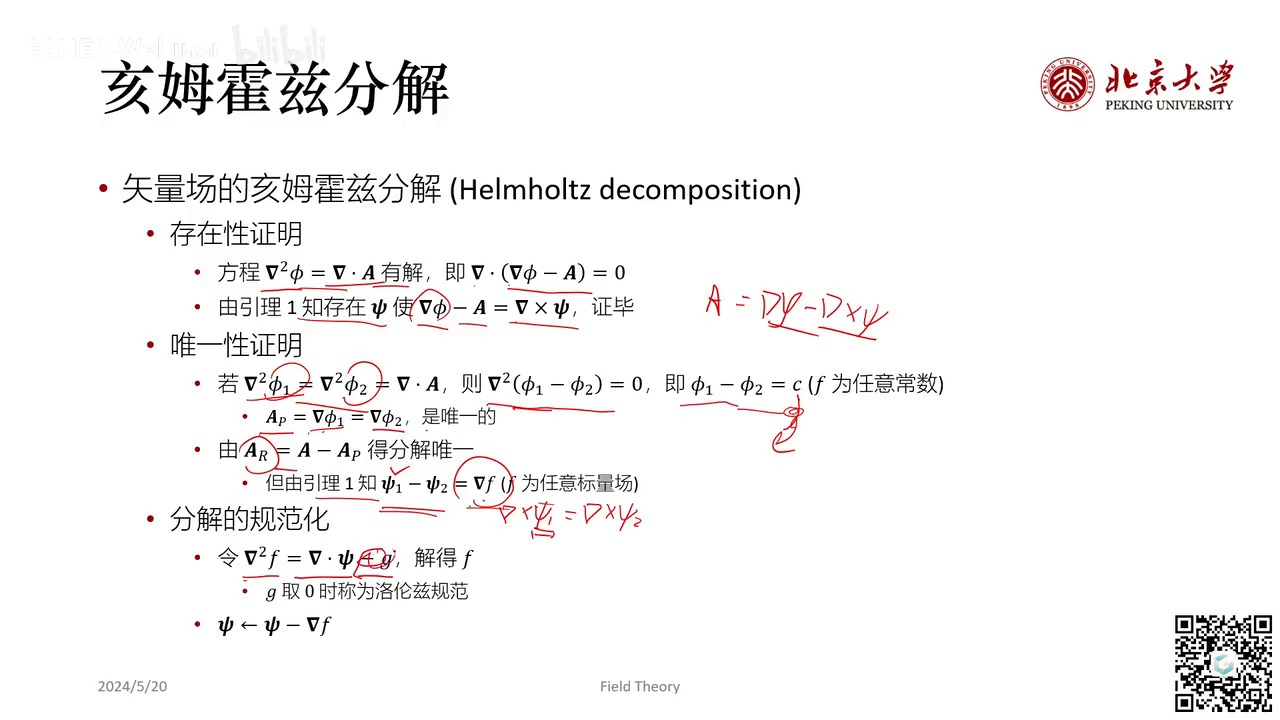
\includegraphics[width=0.92\textwidth]{figures/fig_18_helmholtz_proof.jpg}
\caption{亥姆霍兹分解的存在性、唯一性证明与规范化\vtag}
\end{figure}
\srcnote{00:43:30--00:43:45}
\end{minipage}


\textbf{存在性。}方程 $\nabla^2\phi=\nabla\cdot\boldsymbol A$ 有解，即 $\nabla\cdot(\nabla\phi-\boldsymbol A)=0$。由引理一知存在 $\boldsymbol\psi$ 使 $\nabla\phi-\boldsymbol A=\nabla\times\boldsymbol\psi$，证毕（向量势的符号可以并入 $\boldsymbol\psi$）。

\textbf{唯一性。}若 $\nabla^2\phi_1=\nabla^2\phi_2=\nabla\cdot\boldsymbol A$，则 $\nabla^2(\phi_1-\phi_2)=0$，讲者说在没有给定边界条件的情况下，$\phi_1-\phi_2=c$（$c$ 为任意常数）。于是 $\boldsymbol A_P=\nabla\phi_1=\nabla\phi_2$，是唯一的。再由 $\boldsymbol A_R=\boldsymbol A-\boldsymbol A_P$ 得分解唯一。但由引理一知 $\boldsymbol\psi_1-\boldsymbol\psi_2=\nabla f$（$f$ 为任意标量场），所以分解是唯一的，而势函数不唯一。

\noindent\begin{minipage}{\textwidth}
\begin{figure}[H]
\centering
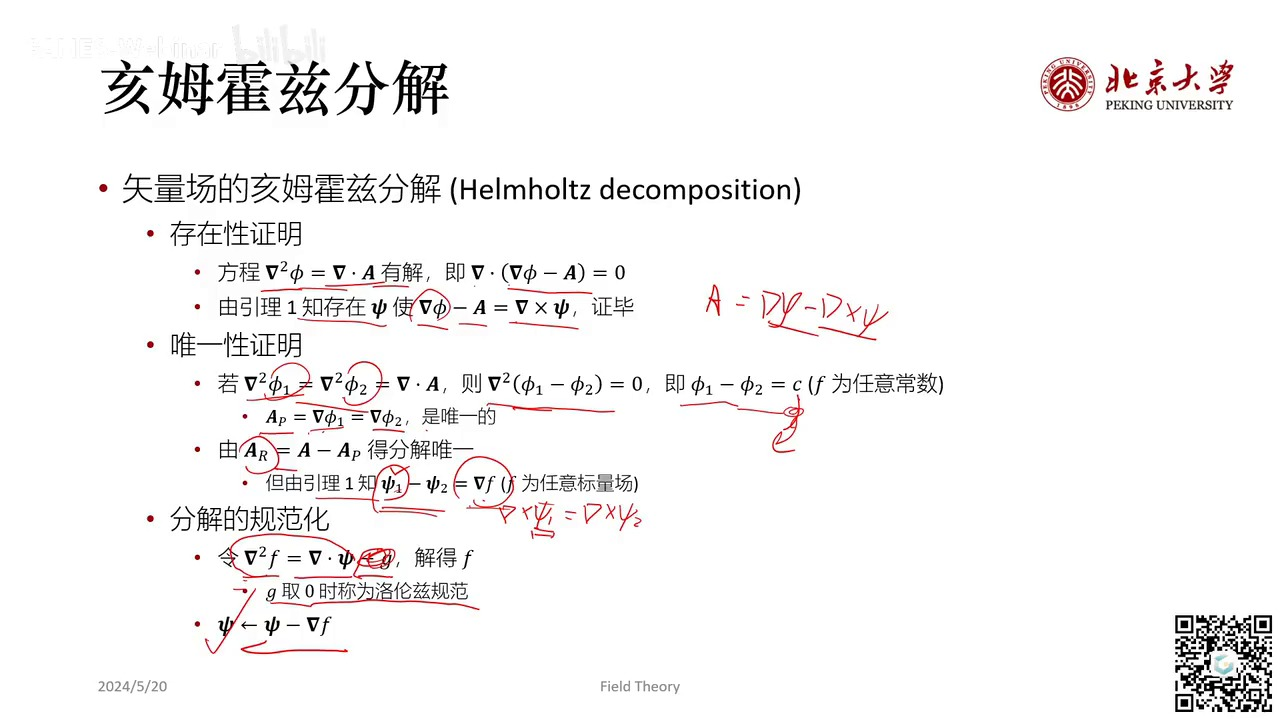
\includegraphics[width=0.92\textwidth]{figures/fig_19_helmholtz_proof_note.jpg}
\caption{讲者在唯一性证明旁的板书\vtag}
\end{figure}
\srcnote{00:44:00--00:44:15}
\end{minipage}


\textbf{规范化。}能不能让势函数也唯一呢？可以。令 $\nabla^2 f=\nabla\cdot\boldsymbol\psi-g$，解得 $f$，然后令 $\boldsymbol\psi\leftarrow\boldsymbol\psi-\nabla f$。$g$ 取零时称为洛伦兹规范。这样向量势 $\boldsymbol\psi$ 也变成了唯一的结果。

\begin{importantbox}{亥姆霍兹分解在图形学中的用处}
讲义作者补充：流体模拟中常用的“投影法”就是亥姆霍兹分解的应用。先不管不可压条件更新速度，得到一个有散的速度场 $\boldsymbol A$；再求解泊松方程 $\nabla^2\phi=\nabla\cdot\boldsymbol A$，减去 $\nabla\phi$，剩下的就是无散部分，满足不可压条件 $\nabla\cdot\boldsymbol u=0$。
\end{importantbox}

\section{外微分}

讲者说，很多刚开始接触矢量分析的同学最头大的地方，在于有很多个公式、很多套运算。有没有一种数学可以概括前面这么多概念？答案是肯定的，这就是外微分，它超出了高等数学的内容。外微分的概念来自积分的定向。

\subsection{积分的定向}

\noindent\begin{minipage}{\textwidth}
\begin{figure}[H]
\centering
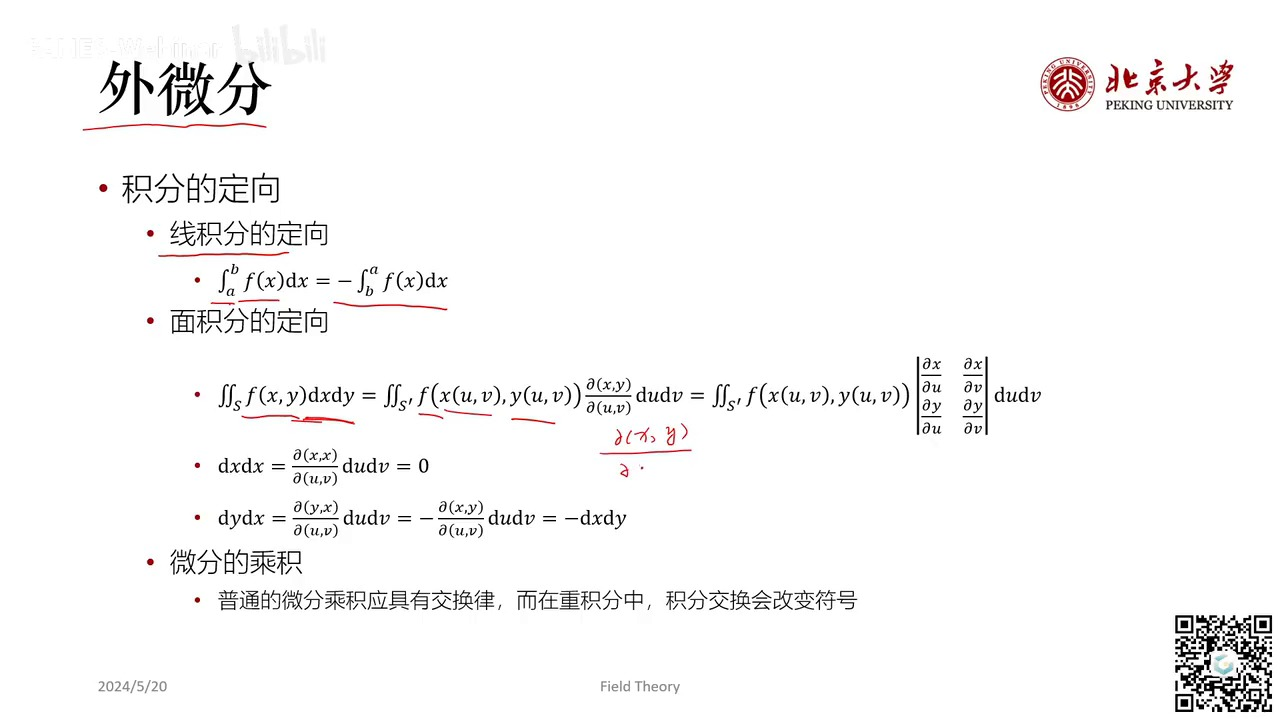
\includegraphics[width=0.92\textwidth]{figures/fig_20_orientation.jpg}
\caption{线积分与面积分的定向\vtag}
\end{figure}
\srcnote{00:47:00--00:47:15}
\end{minipage}


线积分的定向大家都熟悉：
\begin{equation}
\int_a^b f(x)\,\mathrm{d}x=-\int_b^a f(x)\,\mathrm{d}x .
\end{equation}
面积分的定向来自换元。把 $\mathrm{d}x\,\mathrm{d}y$ 换成 $\mathrm{d}u\,\mathrm{d}v$ 时要乘上雅可比行列式：
\begin{equation}
\iint_S f(x,y)\,\mathrm{d}x\,\mathrm{d}y=\iint_{S'}f\big(x(u,v),y(u,v)\big)\frac{\partial(x,y)}{\partial(u,v)}\,\mathrm{d}u\,\mathrm{d}v .
\end{equation}
讲者指出一件很反直觉的事：如果把它写成 $\partial(x,y)/\partial(v,u)$，结果和原来差一个负号。也就是说，在做积分换元时，结果和换元的先后顺序有关。沿着这个思路硬推下去，还会得到 $\mathrm{d}x\,\mathrm{d}x=\frac{\partial(x,x)}{\partial(u,v)}\mathrm{d}u\,\mathrm{d}v=0$，因为两个 $x$ 同时出现在雅可比行列式中，两行相同，行列式为零；以及 $\mathrm{d}y\,\mathrm{d}x=-\mathrm{d}x\,\mathrm{d}y$。普通的微分乘积应该有交换律，而在重积分中，积分交换会改变符号。

\subsection{外积运算}

\noindent\begin{minipage}{\textwidth}
\begin{figure}[H]
\centering
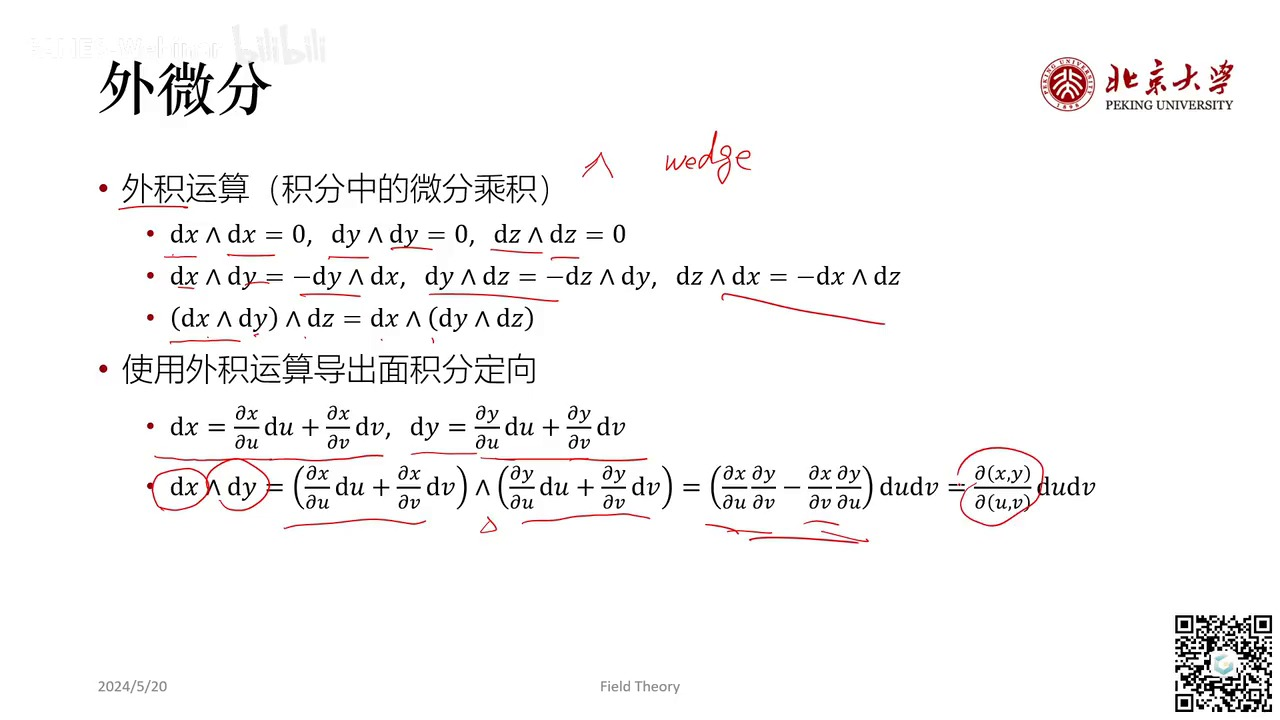
\includegraphics[width=0.92\textwidth]{figures/fig_21_wedge.jpg}
\caption{外积运算及用外积导出面积分定向\vtag}
\end{figure}
\srcnote{00:50:45--00:51:00}
\end{minipage}


有没有运算能表达这种交换性质？这就是外积运算，记作 $\wedge$，英文叫 wedge。定义为
\begin{equation}
\begin{gathered}
\mathrm{d}x\wedge\mathrm{d}x=0,\quad \mathrm{d}y\wedge\mathrm{d}y=0,\quad \mathrm{d}z\wedge\mathrm{d}z=0,\\
\mathrm{d}x\wedge\mathrm{d}y=-\mathrm{d}y\wedge\mathrm{d}x,\quad \mathrm{d}y\wedge\mathrm{d}z=-\mathrm{d}z\wedge\mathrm{d}y,\quad \mathrm{d}z\wedge\mathrm{d}x=-\mathrm{d}x\wedge\mathrm{d}z,\\
(\mathrm{d}x\wedge\mathrm{d}y)\wedge\mathrm{d}z=\mathrm{d}x\wedge(\mathrm{d}y\wedge\mathrm{d}z).
\end{gathered}
\end{equation}
用外积运算可以导出面积分的定向。把 $\mathrm{d}x$、$\mathrm{d}y$ 用链式法则展开为 $\mathrm{d}u$、$\mathrm{d}v$ 的组合，再做外积：
\begin{equation}
\mathrm{d}x\wedge\mathrm{d}y=\left(\frac{\partial x}{\partial u}\mathrm{d}u+\frac{\partial x}{\partial v}\mathrm{d}v\right)\wedge\left(\frac{\partial y}{\partial u}\mathrm{d}u+\frac{\partial y}{\partial v}\mathrm{d}v\right)=\frac{\partial(x,y)}{\partial(u,v)}\,\mathrm{d}u\wedge\mathrm{d}v .
\end{equation}
雅可比行列式就这样自然地出现了。

\subsection{外微分形式}

\noindent\begin{minipage}{\textwidth}
\begin{figure}[H]
\centering
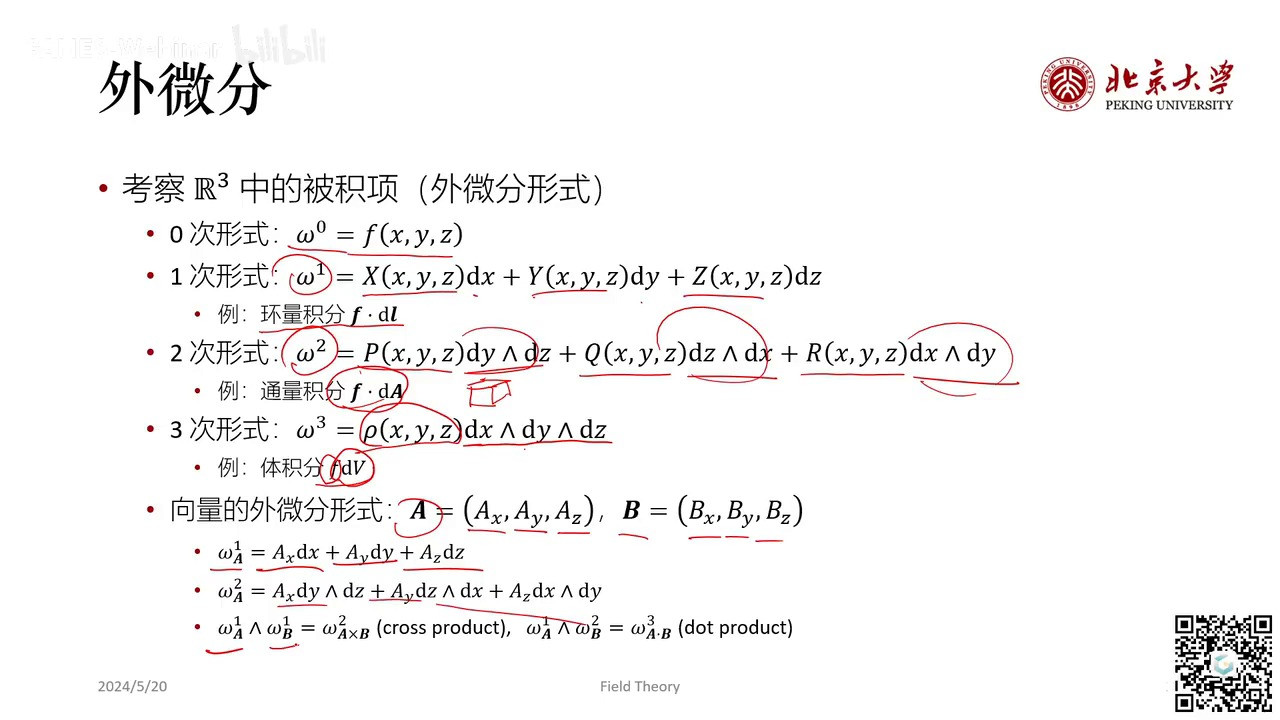
\includegraphics[width=0.92\textwidth]{figures/fig_22_forms.jpg}
\caption{$\mathbb R^3$ 中的被积项：0 到 3 次外微分形式\vtag}
\end{figure}
\srcnote{00:54:00--00:54:15}
\end{minipage}


在 $\mathbb R^3$ 中做积分时，被积项是有规律的，可以按次数整理：
\begin{itemize}
\item 0 次形式：$\omega^0=f(x,y,z)$；
\item 1 次形式：$\omega^1=X\,\mathrm{d}x+Y\,\mathrm{d}y+Z\,\mathrm{d}z$，例如环量积分 $\boldsymbol f\cdot\mathrm{d}\boldsymbol l$；
\item 2 次形式：$\omega^2=P\,\mathrm{d}y\wedge\mathrm{d}z+Q\,\mathrm{d}z\wedge\mathrm{d}x+R\,\mathrm{d}x\wedge\mathrm{d}y$，例如通量积分 $\boldsymbol f\cdot\mathrm{d}\boldsymbol A$；
\item 3 次形式：$\omega^3=\rho\,\mathrm{d}x\wedge\mathrm{d}y\wedge\mathrm{d}z$，例如体积分 $f\,\mathrm{d}V$。
\end{itemize}
对向量 $\boldsymbol A=(A_x,A_y,A_z)$，记它的 1 次形式和 2 次形式为
\begin{equation}
\omega_{\boldsymbol A}^1=A_x\mathrm{d}x+A_y\mathrm{d}y+A_z\mathrm{d}z,\qquad \omega_{\boldsymbol A}^2=A_x\mathrm{d}y\wedge\mathrm{d}z+A_y\mathrm{d}z\wedge\mathrm{d}x+A_z\mathrm{d}x\wedge\mathrm{d}y .
\end{equation}
可以用外积的运算法则验证：$\omega_{\boldsymbol A}^1\wedge\omega_{\boldsymbol B}^1=\omega_{\boldsymbol A\times\boldsymbol B}^2$，即两个向量的 1 次形式做外积得到叉乘的 2 次形式；$\omega_{\boldsymbol A}^1\wedge\omega_{\boldsymbol B}^2=\omega_{\boldsymbol A\cdot\boldsymbol B}^3$，得到点乘的 3 次形式。

\subsection{外微分}

\noindent\begin{minipage}{\textwidth}
\begin{figure}[H]
\centering
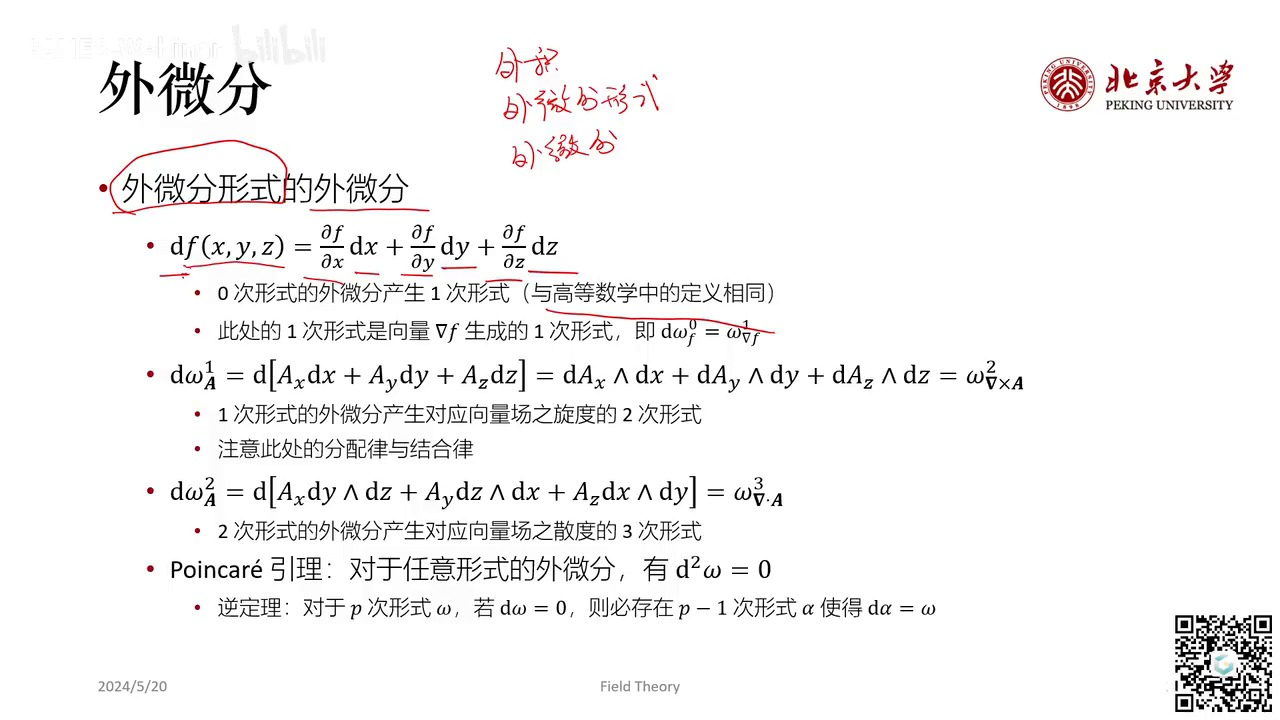
\includegraphics[width=0.92\textwidth]{figures/fig_23_exterior_d.jpg}
\caption{外微分形式的外微分与庞加莱引理\vtag}
\end{figure}
\srcnote{00:56:00--00:56:15}
\end{minipage}


外微分是微分的推广，符号与微分一样写作 $\mathrm{d}$。0 次形式的外微分为
\begin{equation}
\mathrm{d}f=\frac{\partial f}{\partial x}\mathrm{d}x+\frac{\partial f}{\partial y}\mathrm{d}y+\frac{\partial f}{\partial z}\mathrm{d}z,
\end{equation}
与高等数学中的定义完全相同。0 次形式的外微分产生 1 次形式，并且这个 1 次形式正是梯度 $\nabla f$ 生成的 1 次形式，即 $\mathrm{d}\omega_f^0=\omega_{\nabla f}^1$。

对乘积的外微分，与普通微分一样满足莱布尼茨法则，只是中间的乘号改成外积符号。由此计算 1 次形式的外微分：
\begin{equation}
\mathrm{d}\omega_{\boldsymbol A}^1=\mathrm{d}A_x\wedge\mathrm{d}x+\mathrm{d}A_y\wedge\mathrm{d}y+\mathrm{d}A_z\wedge\mathrm{d}z=\omega_{\nabla\times\boldsymbol A}^2 .
\end{equation}
把 $\mathrm{d}A_x$ 再展开成 $\frac{\partial A_x}{\partial x}\mathrm{d}x+\frac{\partial A_x}{\partial y}\mathrm{d}y+\frac{\partial A_x}{\partial z}\mathrm{d}z$，按外积规则整理，就得到 $\boldsymbol A$ 的旋度的 2 次形式。类似地，2 次形式的外微分产生对应向量场散度的 3 次形式，$\mathrm{d}\omega_{\boldsymbol A}^2=\omega_{\nabla\cdot\boldsymbol A}^3$。

\noindent\begin{minipage}{\textwidth}
\begin{figure}[H]
\centering
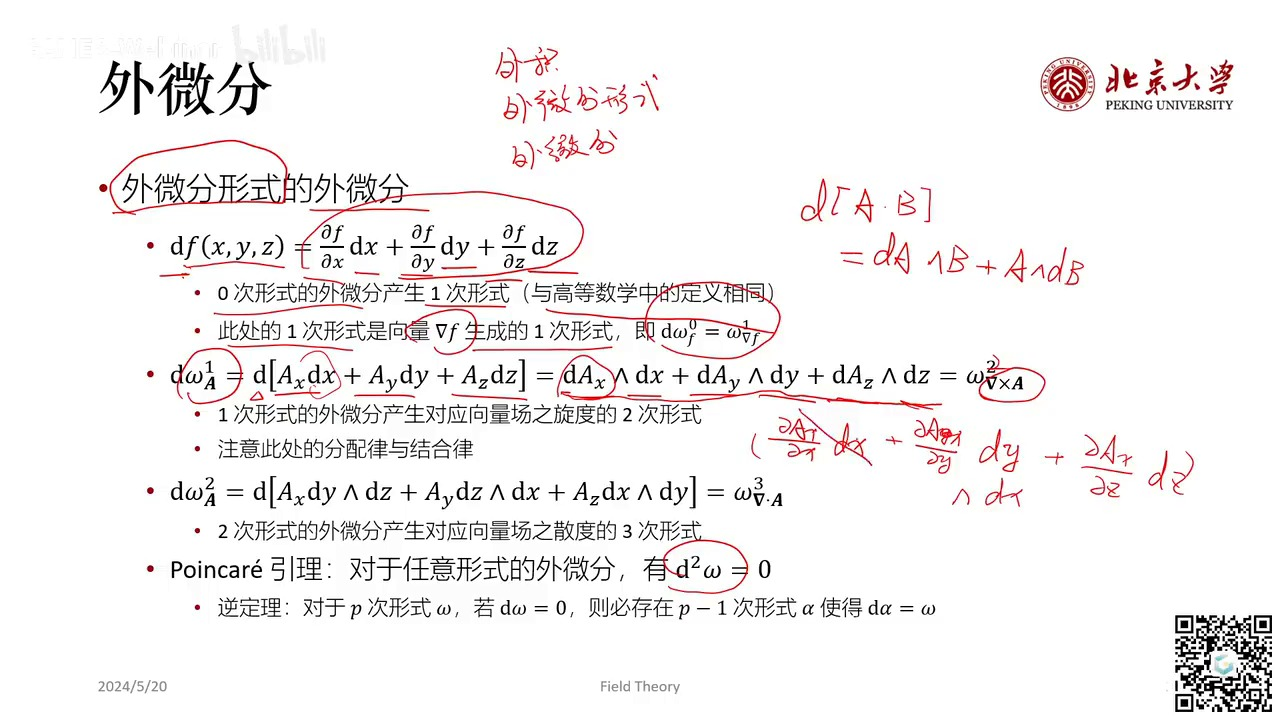
\includegraphics[width=0.92\textwidth]{figures/fig_24_exterior_note.jpg}
\caption{讲者在课件上展开 $\mathrm{d}\omega^1$ 的批注\vtag}
\end{figure}
\srcnote{00:58:45--00:59:00}
\end{minipage}


\begin{knowledgebox}{一张对应表}
外微分把三种“求导”统一了：
\begin{itemize}
\item 0 次形式 $\xrightarrow{\mathrm d}$ 1 次形式：梯度；
\item 1 次形式 $\xrightarrow{\mathrm d}$ 2 次形式：旋度；
\item 2 次形式 $\xrightarrow{\mathrm d}$ 3 次形式：散度。
\end{itemize}
讲者强烈建议从外积和外微分的定义出发，一步一步亲自推导一遍，这样理解会深刻得多。
\end{knowledgebox}

庞加莱（Poincaré）引理：对于任意形式的外微分，有 $\mathrm{d}^2\omega=0$。它还有逆定理：对于 $p$ 次形式 $\omega$，若 $\mathrm{d}\omega=0$，则存在 $p-1$ 次形式 $\alpha$ 使得 $\mathrm{d}\alpha=\omega$。

\subsection{用外微分证明恒等式}

\noindent\begin{minipage}{\textwidth}
\begin{figure}[H]
\centering
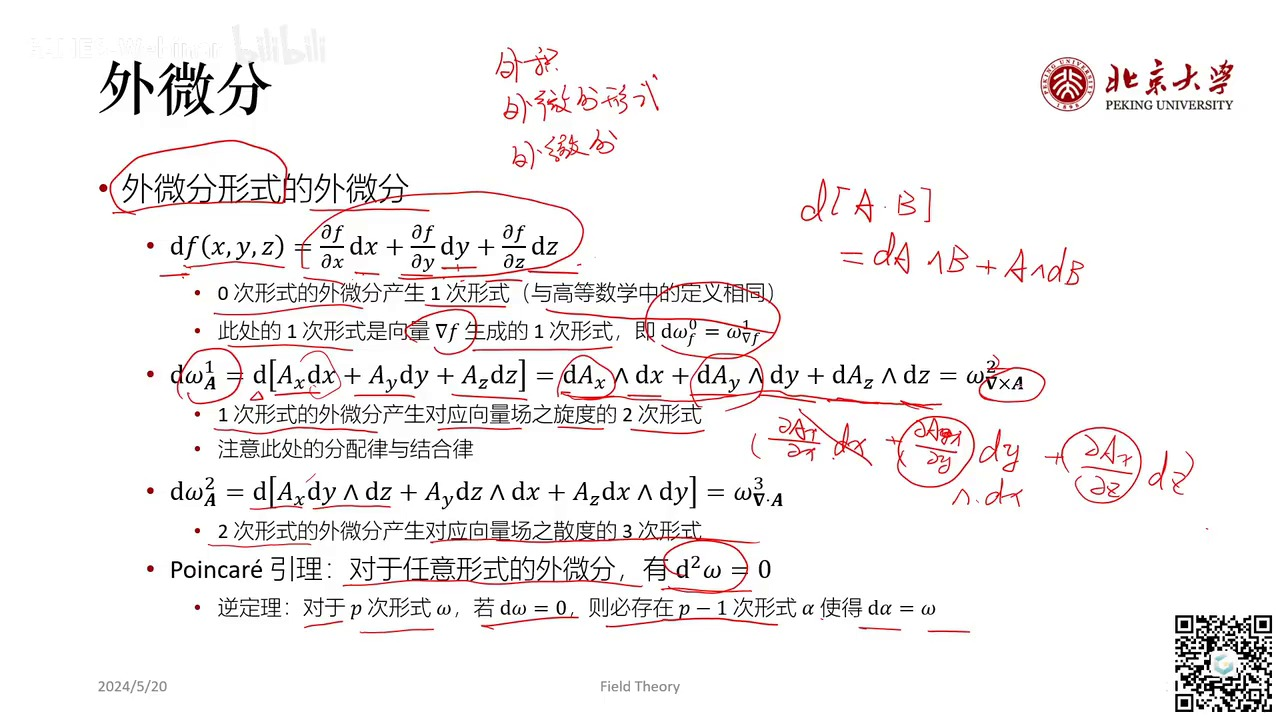
\includegraphics[width=0.92\textwidth]{figures/fig_25_proof_identities.jpg}
\caption{利用外微分证明矢量分析恒等式与外微分形式的斯托克斯公式\vtag}
\end{figure}
\srcnote{01:02:00--01:02:15}
\end{minipage}


外微分的第一个用处是证明矢量分析恒等式。梯度的旋度是先对 $\phi$ 求一次外微分得梯度，再求一次得旋度，即 $\mathrm{d}^2\phi$，由庞加莱引理它等于零；同样，先求旋度再求散度也是 $\mathrm{d}^2$，等于零：
\begin{equation}
\nabla\times\nabla\phi=\boldsymbol 0,\qquad \nabla\cdot(\nabla\times\boldsymbol\psi)=0\quad\Longleftrightarrow\quad \mathrm{d}^2=0 .
\end{equation}
还可以证明多个场函数的恒等式，例如 $\nabla\cdot(\boldsymbol f\times\boldsymbol g)=\boldsymbol g\cdot(\nabla\times\boldsymbol f)-\boldsymbol f\cdot(\nabla\times\boldsymbol g)$。由 $\omega_{\boldsymbol f\times\boldsymbol g}^2=\omega_{\boldsymbol f}^1\wedge\omega_{\boldsymbol g}^1$，两边求外微分：
\begin{equation}
\mathrm{d}(\omega_{\boldsymbol f}^1\wedge\omega_{\boldsymbol g}^1)=\mathrm{d}\omega_{\boldsymbol f}^1\wedge\omega_{\boldsymbol g}^1-\omega_{\boldsymbol f}^1\wedge\mathrm{d}\omega_{\boldsymbol g}^1=\omega_{\nabla\times\boldsymbol f}^2\wedge\omega_{\boldsymbol g}^1-\omega_{\boldsymbol f}^1\wedge\omega_{\nabla\times\boldsymbol g}^2 ,
\end{equation}
再利用 1 次形式与 2 次形式的外积等于点乘的 3 次形式，就得到
\begin{equation}
\omega^3_{\nabla\cdot(\boldsymbol f\times\boldsymbol g)}=\omega^3_{\boldsymbol g\cdot(\nabla\times\boldsymbol f)}-\omega^3_{\boldsymbol f\cdot(\nabla\times\boldsymbol g)} .
\end{equation}

\begin{warningbox}{外微分莱布尼茨法则中的符号}
讲义作者提醒：外微分的乘积法则是 $\mathrm{d}(\alpha\wedge\beta)=\mathrm{d}\alpha\wedge\beta+(-1)^p\alpha\wedge\mathrm{d}\beta$，其中 $p$ 是 $\alpha$ 的次数。对两个 1 次形式，第二项前是负号，这正是上式中减号的来源；直接照搬普通微分的乘积法则会把符号弄错。
\end{warningbox}

\subsection{外微分形式的斯托克斯公式}

外微分最漂亮的结论是外微分形式的斯托克斯公式：
\begin{equation}
\int_{\partial\Omega}\omega=\int_\Omega\mathrm{d}\omega .
\end{equation}
讲者说，之前的高斯公式、格林公式、斯托克斯公式，以及牛顿—莱布尼茨公式，全部都可以写成这一个形式：在积分域的边界上对 $\omega$ 积分，等于在积分域上对 $\mathrm{d}\omega$ 积分。例如高斯公式中，通量积分是 2 次形式，它的外微分是散度的 3 次形式，右边就是散度的体积分；斯托克斯定理说环量积分等于旋度的面积分，环量积分是 1 次形式，旋度的面积分是它外微分得到的 2 次形式。

\begin{practicebox}{自测}
\begin{enumerate}
\item 用 $\nabla$ 的形式写出梯度、散度、旋度和拉普拉斯算子，并说明各自作用在什么场上、得到什么场。
\item 计算 $\boldsymbol F=(x-y)\boldsymbol i+(x+y)\boldsymbol j$ 的散度和旋度，并把它分解成一个无旋场与一个无源场之和。
\item 用外积规则验证 $\mathrm{d}x\wedge\mathrm{d}y$ 换元后出现雅可比行列式。
\item 说明牛顿—莱布尼茨公式为什么是 $\int_{\partial\Omega}\omega=\int_\Omega\mathrm{d}\omega$ 在 0 次形式时的特例。
\end{enumerate}
\end{practicebox}

\section{小结}

讲者最后说，如果不太喜欢外微分这一套运算法则，也可以用本学期第一讲线性代数最后讲的张量运算、指标运算的方法去证明上面的恒等式，只不过更复杂、更缺乏几何直观。如果能熟练运用外微分，它会成为研究定义在场上的问题的有力工具。讲者表示，他个人备课下来的感觉是：仅从应用的角度，从那几条定义出发推导后面的运算并没有困难。

\begin{knowledgebox}{与后续课程的联系}
讲义作者补充：本讲的散度、旋度、拉普拉斯算子和亥姆霍兹分解，是后面偏微分方程、流体模拟和几何处理的基础。例如离散微分几何中的“离散外微分”，正是把本讲的外微分搬到网格上，用来构造离散的梯度、旋度和散度算子。
\end{knowledgebox}

\end{document}
